\documentclass[10pt,letterpaper]{article}
\usepackage[margin=0.72in,headheight=15pt]{geometry}
\usepackage[T1]{fontenc}
\usepackage{lmodern}
\usepackage{microtype}
\usepackage{amsmath,amssymb,mathtools}
\usepackage{booktabs,longtable,array,tabularx}
\usepackage{enumitem}
\usepackage{xcolor}
\usepackage{tikz}
\usetikzlibrary{arrows.meta,calc,fit,positioning,shapes.geometric,backgrounds}
\usepackage{pgfplots}
\pgfplotsset{compat=1.18}
\usepackage{listings}
\usepackage{fancyhdr}
\usepackage{hyperref}
\usepackage{bookmark}

\definecolor{navy}{HTML}{173B57}
\definecolor{blue}{HTML}{2D74A8}
\definecolor{teal}{HTML}{238A8D}
\definecolor{orange}{HTML}{E07A28}
\definecolor{red}{HTML}{C7473A}
\definecolor{green}{HTML}{3F8F63}
\definecolor{gold}{HTML}{D8A52A}
\definecolor{ink}{HTML}{20262E}
\definecolor{muted}{HTML}{66717E}
\definecolor{paper}{HTML}{F7F9FB}
\definecolor{line}{HTML}{D7DEE7}

\hypersetup{
  colorlinks=true,
  linkcolor=navy,
  urlcolor=blue,
  citecolor=navy,
  pdftitle={HS3 Algorithm Technical Documentation},
  pdfauthor={Repository technical documentation updated from commit 8dbdeca}
}
\setlength{\parindent}{0pt}
\setlength{\parskip}{5pt plus 1pt minus 1pt}
\setlength{\emergencystretch}{2em}
\setlist[itemize]{leftmargin=1.35em,itemsep=2pt,topsep=3pt}
\setlist[enumerate]{leftmargin=1.55em,itemsep=3pt,topsep=3pt}
\renewcommand{\arraystretch}{1.12}
\pagestyle{fancy}
\fancyhf{}
\lhead{HS3 technical documentation}
\rhead{\texttt{8dbdeca}}
\cfoot{\thepage}
\setcounter{tocdepth}{2}

\lstdefinestyle{matlabstyle}{
  language=Matlab,
  basicstyle=\ttfamily\footnotesize,
  keywordstyle=\color{navy}\bfseries,
  commentstyle=\color{green},
  stringstyle=\color{orange},
  frame=single,
  rulecolor=\color{line},
  backgroundcolor=\color{paper},
  breaklines=true,
  columns=fullflexible,
  showstringspaces=false,
  numbers=left,
  numberstyle=\tiny\color{muted},
  xleftmargin=1.6em,
  framexleftmargin=1.2em
}
\lstset{style=matlabstyle}

\newcommand{\file}[1]{\nolinkurl{#1}}
\newcommand{\src}[2]{\file{#1}, lines #2}
\newcommand{\term}[1]{\textbf{#1}}
\newcommand{\scriptentry}[2]{%
  \par\medskip\noindent\textbf{\file{#1}}\par
  \begingroup\raggedright #2\par\endgroup
}
\newcommand{\callout}[2]{%
  \begin{center}
  \fcolorbox{#1}{paper}{\begin{minipage}{0.94\linewidth}#2\end{minipage}}
  \end{center}
}

\begin{document}

\begin{titlepage}
\begin{tikzpicture}[remember picture,overlay]
  \fill[navy] (current page.north west) rectangle
    ([yshift=-2.35in]current page.north east);
  \fill[teal] ([yshift=-2.35in]current page.north west) rectangle
    ([yshift=-2.48in]current page.north east);
  \draw[line width=1.2pt]
    ([xshift=0.72in,yshift=0.72in]current page.south west) rectangle
    ([xshift=-0.72in,yshift=-2.82in]current page.north east);
\end{tikzpicture}

\vspace*{0.42in}
{\color{white}\sffamily\bfseries\fontsize{31}{35}\selectfont
HS3 Algorithm\par Technical Documentation}

\vspace{0.24in}
{\color{white}\sffamily\large
Azimuth/elevation obstacle transformation, third-order Hermite-Simpson
transcription, solver flow, validation, and complete MATLAB file reference}

\vspace{1.35in}
\begin{tabular}{@{}ll@{}}
\textbf{Repository branch} & \file{HS3-planner} \\
\textbf{Documented commit} & \file{8dbdeca} \\
\textbf{Snapshot date} & 2026-08-27 \\
\textbf{Scope} & 93 tracked MATLAB files and 17 tracked support artifacts \\
\textbf{Coordinate convention} & Euclidean $[\mathrm{azimuth},\mathrm{elevation}]$ in degrees
\end{tabular}

\vfill
\callout{orange}{
\textbf{Snapshot rule.} This document describes the tracked repository at the
commit above. The untracked \file{Rogue Examples/} directory is intentionally
excluded because it is not part of that commit. No planner behavior was changed
while producing this documentation.}

{\small This is implementation documentation, not a claim of global
completeness or global optimality. The bounded topology portfolio and local
nonlinear solve limitations are stated explicitly in Section~\ref{sec:limits}.}
\end{titlepage}

\tableofcontents
\clearpage

\section{Purpose, scope, and reading map}

This report explains how the repository turns time-indexed protected polygons
in an azimuth/elevation plane into a dynamically feasible, independently
validated trajectory. It covers two related products:

\begin{itemize}
  \item \term{Obstacle-aware Az/El planner}: the public
  \file{obstacleAvoidance.planTrajectory} API, its geometry/search layer, its
  planner-specific corridor constraints, and its independent collision
  validator.
  \item \term{Dimension-neutral HS3 engine}: the public
  \file{solveTrajHS3} boundary-value solver and the shared
  \file{hs3Internal} polynomial, constraint, and numerical solver components.
\end{itemize}

The obstacle-aware planner deliberately does not call the public
\file{solveTrajHS3} wrapper. It calls the neutral \file{hs3Internal}
primitives through its own adapter because moving/deforming obstacle
associations, route topology, relinearization, and adaptive polygon collision
validation belong to the Az/El layer. This is an architectural boundary, not a
duplicate implementation.

The recommended reading order is: architecture (Section~\ref{sec:architecture}),
mathematics (Section~\ref{sec:math}), obstacle transformation
(Section~\ref{sec:obstacles}), the worked example
(Section~\ref{sec:walkthrough}), and finally the exhaustive file catalog
(Section~\ref{sec:inventory}).

\subsection{Evidence convention}

Source references name a tracked file and line range from commit
\file{ce0dfdd42c5cf186761603fa18d14c5ba4583551}. Mathematical equations are
restatements of implemented formulas. Illustrative numeric values in the
walkthrough are explicitly marked as hand-calculated examples; they are not
presented as measured optimizer output. The repository commit is the primary
authority for implementation-specific claims in this report\cite{repoCommit};
external publications are cited where they explain the underlying method, but
they do not establish what this particular implementation does.

\section{System architecture}\label{sec:architecture}

\subsection{Two-product ownership model}

\begin{figure}[ht]
\centering
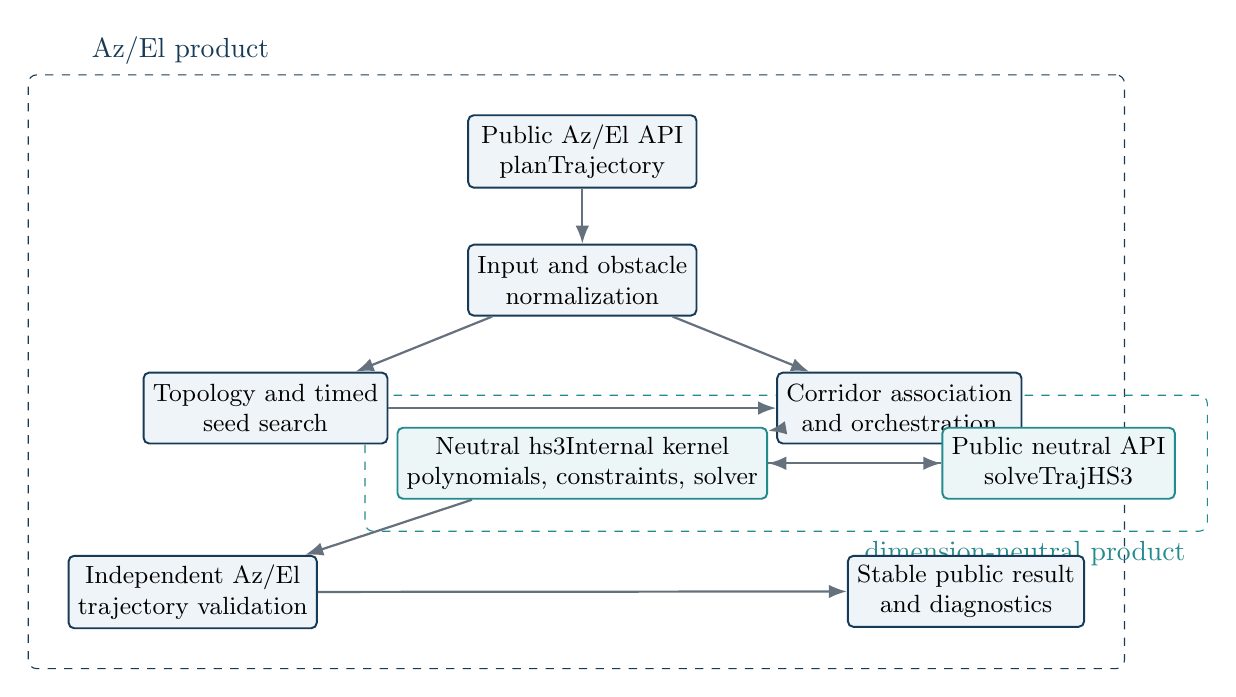
\begin{tikzpicture}[
  node distance=7mm and 10mm,
  box/.style={draw,line width=.7pt,rounded corners=2pt,align=center,
    minimum height=9mm,minimum width=29mm,font=\small,fill=paper},
  prod/.style={box,draw=navy,fill=blue!8},
  neutral/.style={box,draw=teal,fill=teal!8},
  arrow/.style={-{Latex[length=2.3mm]},line width=.8pt,draw=muted}
]
\node[prod] (api) {Public Az/El API\\\file{planTrajectory}};
\node[prod,below=of api] (input) {Input and obstacle\\normalization};
\node[prod,below left=of input] (search) {Topology and timed\\seed search};
\node[prod,below right=of input] (planner) {Corridor association\\and orchestration};
\node[neutral,below=14mm of input] (kernel) {Neutral \file{hs3Internal} kernel\\polynomials, constraints, solver};
\node[prod,below left=of kernel] (valid) {Independent Az/El\\trajectory validation};
\node[prod,below right=of kernel] (result) {Stable public result\\and diagnostics};
\node[neutral,right=22mm of kernel] (standalone) {Public neutral API\\\file{solveTrajHS3}};
\draw[arrow] (api)--(input);
\draw[arrow] (input)--(search);
\draw[arrow] (input)--(planner);
\draw[arrow] (search)--(planner);
\draw[arrow] (planner)--(kernel);
\draw[arrow] (kernel)--(valid);
\draw[arrow] (valid)--(result);
\draw[arrow] (standalone)--(kernel);
\draw[arrow] (kernel)--(standalone);
\begin{scope}[on background layer]
  \node[draw=navy,dashed,rounded corners=3pt,fit=(api)(input)(search)(planner)(valid)(result),
    inner sep=5mm,label={[navy]above left:Az/El product}] {};
  \node[draw=teal,dashed,rounded corners=3pt,fit=(kernel)(standalone),
    inner sep=4mm,label={[teal]below right:dimension-neutral product}] {};
\end{scope}
\end{tikzpicture}
\caption{Ownership and dependency direction. Polygon semantics never enter the
neutral HS3 source. The public neutral wrapper and the Az/El planner share the
same kernel but have different orchestration and validation responsibilities.}
\label{fig:architecture}
\end{figure}

\subsection{Public planner contract}

The maintained public call is:

\begin{lstlisting}
result = obstacleAvoidance.planTrajectory( ...
    obstacles, initialState, goalState, limits, options);
\end{lstlisting}

The input roles are fixed and ordered:

\begin{itemize}
  \item \file{obstacles}: canonical static or time-indexed protected polygon
  records, a nested cell/array accepted by the combiner, or empty.
  \item \file{initialState}: absolute \file{time_s} and a 1-by-2
  \file{position_deg}; optional endpoint velocity and acceleration default to
  zero.
  \item \file{goalState}: fixed or sampled moving target with the same
  coordinate ordering and supported terminal derivatives.
  \item \file{limits}: per-axis velocity, acceleration, and jerk limits plus
  optional workspace intervals.
  \item \file{options}: algorithm and runtime controls. Partial structures are
  accepted; defaults have one owner.
\end{itemize}

Expected planning outcomes do not throw. They return one stable schema with
\file{Success=false}, an actionable \file{Message}, a machine-readable
\file{TerminationReason}, resolved inputs/options, search evidence, candidate
summaries, validation, and timing. Invalid input contracts throw identified
errors.

\subsection{End-to-end planner flow}

\begin{figure}[!htbp]
\centering
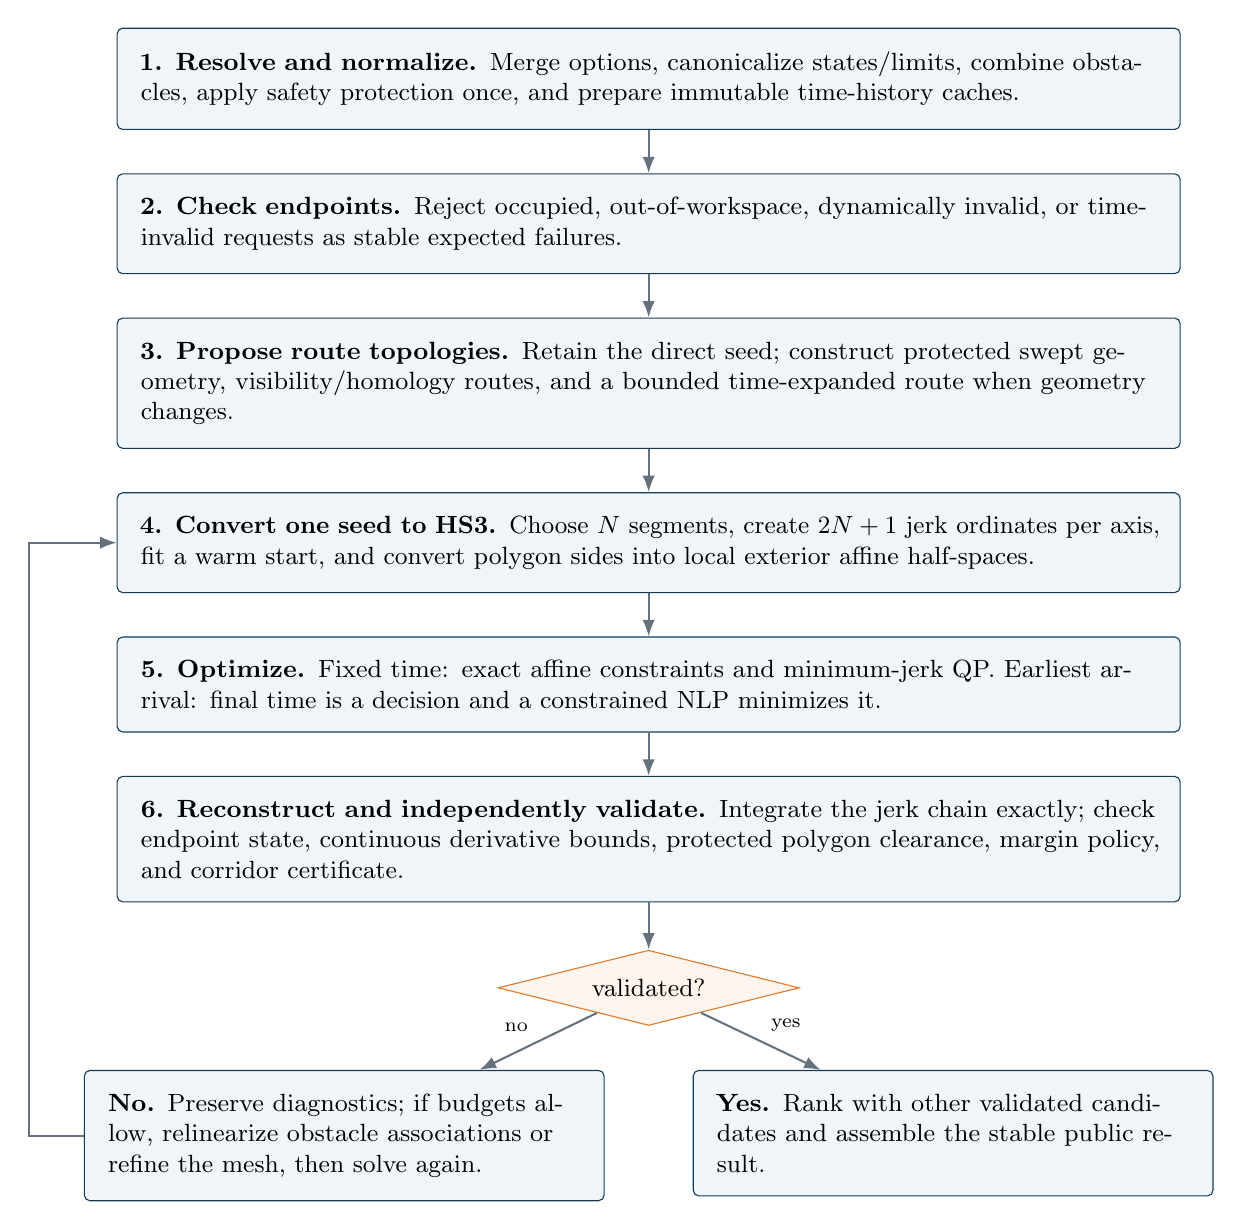
\begin{tikzpicture}[
  node distance=5.5mm,
  stage/.style={draw=navy,fill=blue!7,rounded corners=2pt,align=left,
    text width=12.9cm,minimum height=9mm,inner sep=3mm,font=\small},
  decision/.style={draw=orange,fill=orange!8,diamond,aspect=4.0,align=center,
    inner sep=1.5mm,font=\small},
  arr/.style={-{Latex[length=2.1mm]},draw=muted,line width=.75pt}
]
\node[stage] (s1) {\textbf{1. Resolve and normalize.}
Merge options, canonicalize states/limits, combine obstacles, apply safety
protection once, and prepare immutable time-history caches.};
\node[stage,below=of s1] (s2) {\textbf{2. Check endpoints.}
Reject occupied, out-of-workspace, dynamically invalid, or time-invalid
requests as stable expected failures.};
\node[stage,below=of s2] (s3) {\textbf{3. Propose route topologies.}
Retain the direct seed; construct protected swept geometry, visibility/homology
routes, and a bounded time-expanded route when geometry changes.};
\node[stage,below=of s3] (s4) {\textbf{4. Convert one seed to HS3.}
Choose $N$ segments, create $2N+1$ jerk ordinates per axis, fit a warm start,
and convert polygon sides into local exterior affine half-spaces.};
\node[stage,below=of s4] (s5) {\textbf{5. Optimize.}
Fixed time: exact affine constraints and minimum-jerk QP. Earliest arrival:
final time is a decision and a constrained NLP minimizes it.};
\node[stage,below=of s5] (s6) {\textbf{6. Reconstruct and independently validate.}
Integrate the jerk chain exactly; check endpoint state, continuous derivative
bounds, protected polygon clearance, margin policy, and corridor certificate.};
\node[decision,below=6mm of s6] (ok) {validated?};
\node[stage,below left=8mm and -4mm of ok,text width=6.0cm] (refine)
{\textbf{No.} Preserve diagnostics; if budgets allow, relinearize obstacle
associations or refine the mesh, then solve again.};
\node[stage,below right=8mm and -4mm of ok,text width=6.0cm] (accept)
{\textbf{Yes.} Rank with other validated candidates and assemble the stable
public result.};
\draw[arr] (s1)--(s2); \draw[arr] (s2)--(s3); \draw[arr] (s3)--(s4);
\draw[arr] (s4)--(s5); \draw[arr] (s5)--(s6); \draw[arr] (s6)--(ok);
\draw[arr] (ok)--node[above left,font=\scriptsize]{no}(refine);
\draw[arr] (ok)--node[above right,font=\scriptsize]{yes}(accept);
\draw[arr] (refine.west) -- ++(-7mm,0) |- (s4.west);
\end{tikzpicture}
\caption{The maintained obstacle-aware planning sequence. Search proposals and
optimizer feasibility are not accepted as proof; independent validation is the
authority.}
\label{fig:plannerflow}
\end{figure}

\section{HS3 mathematical formulation}\label{sec:math}

\subsection{What HS3 means in this repository}

The repository explicitly calls the method a \term{third-order
Hermite-Simpson (HS3) transcription}. Its separated higher-order state-chain
interpretation is consistent with the collocation formulation discussed by
Moreno-Martin, Ros, and Celaya\cite{moreno2024}. For $D$ coordinates and $N$
equal-time segments, the implemented decision is a shared chain of jerk
ordinates

\begin{equation}
J = \{j_0,j_{1/2},j_1,j_{3/2},\ldots,j_N\}
\in \mathbb{R}^{(2N+1)\times D}.
\end{equation}

For earliest-arrival problems, the absolute final time $t_f$ is appended to
the decision vector. For fixed arrival, $t_f$ is data and the jerk controls are
the only decisions. Adjacent segments share their endpoint jerk ordinate.

On segment $k$, let $\sigma\in[0,1]$ be local normalized time and let
$h=(t_f-t_0)/N$. If $j_s$, $j_m$, and $j_e$ are the segment start, midpoint,
and end jerk ordinates, the implemented quadratic jerk is

\begin{equation}\label{eq:jerk}
j_k(\sigma)=j_s+(-3j_s+4j_m-j_e)\sigma
 +(2j_s-4j_m+2j_e)\sigma^2.
\end{equation}

This is exactly the formula in
\src{hs3/+hs3Internal/+polynomial/createTrajectoryPolynomial.m}{31-35}.
Exact integration with the inherited state at the beginning of the segment
produces cubic acceleration, quartic velocity, and quintic position. State is
propagated from one segment to the next, so position, velocity, and
acceleration remain continuous.

\begin{figure}[ht]
\centering
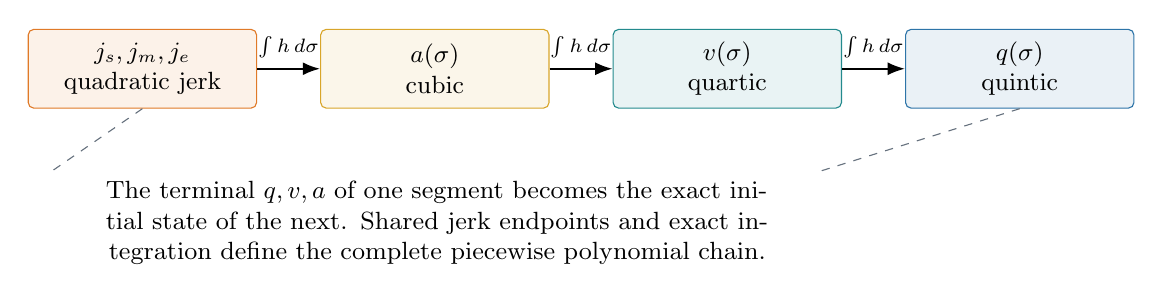
\begin{tikzpicture}[
  node distance=8mm,
  b/.style={draw,rounded corners=2pt,minimum width=29mm,minimum height=10mm,
    align=center,font=\small},
  a/.style={-{Latex[length=2.2mm]},line width=.8pt}
]
\node[b,draw=orange,fill=orange!10] (J) {$j_s,j_m,j_e$\\quadratic jerk};
\node[b,draw=gold,fill=gold!10,right=of J] (A) {$a(\sigma)$\\cubic};
\node[b,draw=teal,fill=teal!10,right=of A] (V) {$v(\sigma)$\\quartic};
\node[b,draw=blue,fill=blue!10,right=of V] (P) {$q(\sigma)$\\quintic};
\draw[a] (J)--node[above,font=\scriptsize]{$\int h\,d\sigma$}(A);
\draw[a] (A)--node[above,font=\scriptsize]{$\int h\,d\sigma$}(V);
\draw[a] (V)--node[above,font=\scriptsize]{$\int h\,d\sigma$}(P);
\node[below=8mm of A,align=center,font=\small,text width=95mm] (state)
{The terminal $q,v,a$ of one segment becomes the exact initial state of the
next. Shared jerk endpoints and exact integration define the complete
piecewise polynomial chain.};
\draw[dashed,muted] (J.south)--(state.north west);
\draw[dashed,muted] (P.south)--(state.north east);
\end{tikzpicture}
\caption{Polynomial orders created by the HS3 control-jerk representation.}
\end{figure}

\subsection{Fixed-time objective and affine structure}

For fixed duration, position, velocity, acceleration, jerk, and terminal state
are affine functions of the jerk vector. The repository builds those maps
directly in \file{createAffineSensitivityModel.m}. The exact integrated
squared-jerk objective for one coordinate and one segment is

\begin{equation}\label{eq:jerkcost}
I_k=\frac{h}{30}\left(
4j_s^2+16j_m^2+4j_e^2+4j_sj_m-2j_sj_e+4j_mj_e
\right).
\end{equation}

Summing Equation~\eqref{eq:jerkcost} over segments and axes produces a
positive semidefinite quadratic objective with an exact gradient and Hessian.
Endpoint constraints and all fixed-time Bernstein/path constraints are affine
in $J$. The neutral fixed-time engine therefore solves a convex quadratic
program with \file{quadprog}\cite{mathworksQuadprog}. The obstacle-aware
adapter uses the same mathematical structure once its local half-space
associations are frozen.

\subsection{Earliest-arrival objective}

For earliest arrival, $t_f$ changes $h$, which changes every integrated
coefficient map, obstacle event coordinate, and continuous bound. The objective
is simply

\begin{equation}
\min_{J,t_f} t_f.
\end{equation}

Jerk derivatives of the constraints remain exact. The final-time derivative is
computed by a safeguarded finite difference that stays within allowed time and
obstacle-event bounds. The local nonlinear problem is solved with
\file{fmincon}\cite{mathworksFmincon}. The engine first obtains a fixed-horizon
seed; if the primary solve is not feasible it may run a bounded
feasibility-recovery stage.

\subsection{Continuous bounds through Bernstein coefficients}

Every segment polynomial is stored in ascending power form. For continuous
position, velocity, acceleration, jerk, and affine corridor checks, the code
converts the relevant polynomial to Bernstein form on the full segment or an
owned subinterval. The complete-interval argument uses the Bernstein
convex-hull property\cite{farouki2012}. If a scalar polynomial is written

\begin{equation}
f(\sigma)=\sum_{r=0}^{d}\beta_r B_{r,d}(\sigma),
\end{equation}

then the Bernstein convex-hull property gives

\begin{equation}
\min_r\beta_r \le f(\sigma)\le \max_r\beta_r,
\qquad \sigma\in[0,1].
\end{equation}

Thus checking every $\beta_r$ against an upper/lower limit certifies the
complete polynomial interval, not only a sampling grid. Subinterval maps are
exact and are restricted to one HS3 segment.

\subsection{Power-to-Bernstein conversion in detail}

The conversion is a change of basis; it does not approximate or resample the
polynomial. Let the ascending-power record for one segment be

\begin{equation}
p(\sigma)=\sum_{k=0}^{d}a_k\sigma^k,
\qquad 0\le\sigma\le1.
\end{equation}

Using

\begin{equation}
\sigma^k=\frac{1}{\binom{d}{k}}
\sum_{i=k}^{d}\binom{i}{k}B_{i,d}(\sigma),
\end{equation}

the same polynomial has Bernstein coefficients

\begin{equation}\label{eq:powerbernstein}
\boxed{\displaystyle
\beta_i=\sum_{k=0}^{i}
\frac{\binom{i}{k}}{\binom{d}{k}}a_k},
\qquad i=0,\ldots,d.
\end{equation}

Equation~\eqref{eq:powerbernstein} is exactly the lower-triangular conversion
assembled by the following implementation owner:

\begin{quote}\small
\file{hs3/+hs3Internal/+polynomial/convertPowerToBernstein.m}, lines 26--38.
\end{quote}

MATLAB's lower-triangular Pascal matrix supplies $\binom{i}{k}$ and columnwise
division by its last row supplies $\binom{d}{k}^{-1}$. The matrix is cached by
degree because position, velocity, acceleration, jerk, sensitivities, and
corridor projections repeatedly use the same basis change.

For a concrete quintic example,

\begin{equation}
p(\sigma)=1+2\sigma-3\sigma^2+0.5\sigma^5,
\quad
a=[1,2,-3,0,0,0.5]^T.
\end{equation}

Applying Equation~\eqref{eq:powerbernstein} gives

\begin{equation}
\beta=[1,1.4,1.5,1.3,0.8,0.5]^T.
\end{equation}

The negative power coefficient $a_2=-3$ does not mean the curve reaches
$-3$; raw power coefficients are not geometric control values. In contrast,
the Bernstein coefficients prove $0.5\le p(\sigma)\le1.5$ over the entire
interval. The bound can be conservative - the curve need not attain either
extreme - but it is continuous and cannot miss a between-sample peak.

\begin{figure}[ht]
\centering
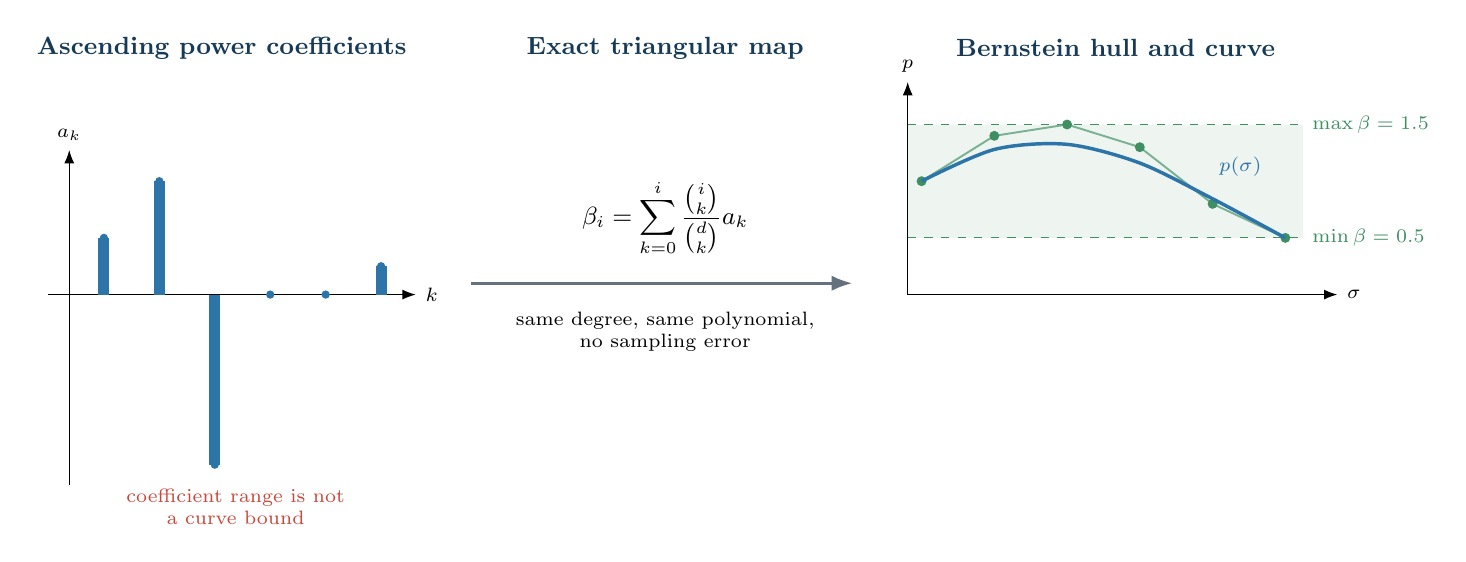
\begin{tikzpicture}[x=0.88cm,y=0.72cm,>=Latex]
\begin{scope}
  \node[font=\bfseries\small,navy] at (2.5,4.35)
    {Ascending power coefficients};
  \draw[->] (0,0)--(5.3,0) node[right,font=\scriptsize]{$k$};
  \draw[->] (.3,-3.35)--(.3,2.55) node[above,font=\scriptsize]{$a_k$};
  \foreach \x/\v in {.8/1,1.6/2,2.4/-3,3.2/0,4.0/0,4.8/.5}{
    \draw[blue,line width=4pt] (\x,0)--(\x,\v);
    \fill[blue] (\x,\v) circle (1.5pt);
  }
  \node[red,font=\scriptsize,align=center] at (2.7,-3.75)
    {coefficient range is not\\a curve bound};
\end{scope}

\begin{scope}[shift={(6.3,0)}]
  \node[font=\bfseries\small,navy] at (2.6,4.35) {Exact triangular map};
  \node[align=center,font=\small] at (2.6,1.35)
    {$\displaystyle \beta_i=\sum_{k=0}^{i}
      \frac{\binom{i}{k}}{\binom{d}{k}}a_k$};
  \draw[->,line width=1pt,muted] (-.2,.2)--(5.3,.2);
  \node[font=\scriptsize,align=center] at (2.6,-.65)
    {same degree, same polynomial,\\no sampling error};
\end{scope}

\begin{scope}[shift={(12.4,0)}]
  \node[font=\bfseries\small,navy] at (3.0,4.35)
    {Bernstein hull and curve};
  \draw[->] (0,0)--(6.2,0) node[right,font=\scriptsize]{$\sigma$};
  \draw[->] (0,0)--(0,3.75) node[above,font=\scriptsize]{$p$};
  \fill[green!9] (0,1.0) rectangle (5.7,3.0);
  \draw[green,dashed] (0,1.0)--(5.7,1.0)
    node[right,font=\scriptsize]{$\min\beta=0.5$};
  \draw[green,dashed] (0,3.0)--(5.7,3.0)
    node[right,font=\scriptsize]{$\max\beta=1.5$};
  \draw[green!70,line width=.7pt]
    plot coordinates {(.2,2.0) (1.25,2.8) (2.3,3.0)
      (3.35,2.6) (4.4,1.6) (5.45,1.0)};
  \foreach \x/\y in {.2/2.0,1.25/2.8,2.3/3.0,3.35/2.6,4.4/1.6,5.45/1.0}
    \fill[green] (\x,\y) circle (1.8pt);
  \draw[blue,line width=1.25pt] plot[smooth] coordinates
    {(.2,2.0) (1.25,2.56) (2.3,2.65) (3.35,2.32)
      (4.4,1.69) (5.45,1.0)};
  \node[blue,font=\scriptsize] at (4.8,2.25) {$p(\sigma)$};
\end{scope}
\end{tikzpicture}
\caption{Exact power-to-Bernstein conversion for the worked quintic. The raw
power coefficients on the left are algebraic coefficients; the Bernstein
coefficients on the right are geometric control values whose convex hull
contains the complete curve.}
\label{fig:powerbernstein}
\end{figure}

For a constraint that owns only $\tau\in[\tau_a,\tau_b]$ inside one HS3
segment, \file{createSubintervalBernsteinMap.m} first substitutes
$\sigma=\sigma_a+(\sigma_b-\sigma_a)u$, $u\in[0,1]$, to obtain an exact power
record on that subinterval, then applies the same conversion. A point row
($\tau_a=\tau_b$) needs one evaluated value; a nonzero interval emits all
$d+1$ Bernstein inequalities. Intervals are prohibited from crossing an HS3
segment boundary so one polynomial record always owns the complete proof.

In the fixed-time problem, the power coefficients are affine in jerk. The code
therefore applies the same triangular basis map to the coefficient
\emph{sensitivity matrices}, not just to one trial curve. This yields exact
linear inequality rows for \file{quadprog}; the solver does not numerically
differentiate those jerk columns.

\subsection{Endpoint and path constraints}

The terminal equality is

\begin{equation}
q(t_f)=q_f,\qquad v(t_f)=v_f,\qquad a(t_f)=a_f.
\end{equation}

The neutral public path-constraint row has fields
\file{Tau}, \file{TauEnd}, \file{Normal}, and \file{LowerBound}. A point row
enforces

\begin{equation}\label{eq:pathrow}
n^T q(\tau)\ge \ell,
\end{equation}

while $\mathrm{TauEnd}>\mathrm{Tau}$ applies the same half-space throughout the
interval using its Bernstein hull. The Az/El planner constructs the equivalent
rows internally from obstacle geometry.

\section{Create 1D, 2D, and 3D HS3 inputs}\label{sec:dimensionexamples}

The neutral \file{solveTrajHS3} function uses the width of the state vectors to
find the number of coordinates. Use a row with $D$ values for every state and
limit that changes by coordinate. A 1D input has one value, a 2D input has two
values, and a 3D input has three values. Do not mix widths in one request.

\begin{center}
\begin{tabularx}{0.96\linewidth}{@{}lX@{}}
\toprule
Input & Required contents \\
\midrule
\file{initialState} & Scalar structure with \file{time}, \file{position},
\file{velocity}, and \file{acceleration}. The three motion fields are
$1\times D$ rows. \\
\file{terminalState} & Scalar structure with \file{position}, \file{velocity},
\file{acceleration}, and \file{maximumTime}. The motion fields are
$1\times D$ rows. \\
\file{limits} & Positive \file{maximumVelocity},
\file{maximumAcceleration}, and \file{maximumJerk}. Each value can be one
scalar for all coordinates or a $1\times D$ row. \\
\file{options} & Use \file{TimeMode="fixed"} and set \file{FinalTime} for a
fixed-duration example. Use \file{TimeMode="free"} to let HS3 find an early
arrival before \file{terminalState.maximumTime}. \\
\bottomrule
\end{tabularx}
\end{center}

All examples below start and finish at rest. They use generous limits so that
the input layout is easy to see. Each example checks \file{trajectory.Success}
and prints the machine-readable termination reason when the solve fails.

\subsection{1D example: move one coordinate}

Use one value in each motion row. This example moves from 0 to 1 in four
seconds.

\begin{lstlisting}
addpath("hs3");

initialState = struct( ...
    "time", 0, ...
    "position", 0, ...
    "velocity", 0, ...
    "acceleration", 0);

terminalState = struct( ...
    "position", 1, ...
    "velocity", 0, ...
    "acceleration", 0, ...
    "maximumTime", 4);

limits = struct( ...
    "maximumVelocity", 2, ...
    "maximumAcceleration", 3, ...
    "maximumJerk", 8);

options = struct("TimeMode", "fixed", "FinalTime", 4);
trajectory = solveTrajHS3( ...
    initialState, terminalState, limits, options);

assert(trajectory.Success, trajectory.Message);
plot(trajectory.time, trajectory.position(:, 1));
xlabel("Time");
ylabel("Coordinate 1");
\end{lstlisting}

The returned histories have one column. For example,
\file{trajectory.position(:,1)} is the complete position history for the only
coordinate.

\subsection{2D example: move two coordinates}

Use two values in each motion row. The first column is coordinate 1. The second
column is coordinate 2. This example moves to $[1,2]$ in five seconds.

\begin{lstlisting}
addpath("hs3");

initialState = struct( ...
    "time", 0, ...
    "position", [0 0], ...
    "velocity", [0 0], ...
    "acceleration", [0 0]);

terminalState = struct( ...
    "position", [1 2], ...
    "velocity", [0 0], ...
    "acceleration", [0 0], ...
    "maximumTime", 5);

limits = struct( ...
    "maximumVelocity", [2 2], ...
    "maximumAcceleration", [3 3], ...
    "maximumJerk", [8 8]);

options = struct("TimeMode", "fixed", "FinalTime", 5);
trajectory = solveTrajHS3( ...
    initialState, terminalState, limits, options);

assert(trajectory.Success, trajectory.Message);
plot(trajectory.position(:, 1), trajectory.position(:, 2));
xlabel("Coordinate 1");
ylabel("Coordinate 2");
axis equal;
\end{lstlisting}

For azimuth/elevation work, coordinate 1 can be azimuth and coordinate 2 can be
elevation. The neutral HS3 function does not assign those meanings. The caller
must use consistent units and coordinate order.

\subsection{3D example: move three coordinates}

Use three values in each motion row. This example moves to
$[1,-1,0.5]$ in six seconds.

\begin{lstlisting}
addpath("hs3");

initialState = struct( ...
    "time", 0, ...
    "position", [0 0 0], ...
    "velocity", [0 0 0], ...
    "acceleration", [0 0 0]);

terminalState = struct( ...
    "position", [1 -1 0.5], ...
    "velocity", [0 0 0], ...
    "acceleration", [0 0 0], ...
    "maximumTime", 6);

limits = struct( ...
    "maximumVelocity", [2 2 2], ...
    "maximumAcceleration", [3 3 3], ...
    "maximumJerk", [8 8 8]);

options = struct("TimeMode", "fixed", "FinalTime", 6);
trajectory = solveTrajHS3( ...
    initialState, terminalState, limits, options);

assert(trajectory.Success, trajectory.Message);
plot3(trajectory.position(:, 1), ...
    trajectory.position(:, 2), ...
    trajectory.position(:, 3));
xlabel("Coordinate 1");
ylabel("Coordinate 2");
zlabel("Coordinate 3");
axis equal;
\end{lstlisting}

The returned position, velocity, acceleration, and jerk histories have three
columns. The row count is the number of returned time samples.

\subsection{Change limits by coordinate}

A scalar limit applies to all coordinates. A row gives each coordinate its own
limit. For example, the following 3D limits allow coordinate 1 to move faster
than coordinates 2 and 3:

\begin{lstlisting}
limits.maximumVelocity = [4 2 1];
limits.maximumAcceleration = [6 3 2];
limits.maximumJerk = [12 8 4];
\end{lstlisting}

If input validation reports a size error, compare the width of every position,
velocity, acceleration, limit, and path-normal row. They must all describe the
same value of $D$. If the sizes are correct but no motion is found, inspect
\file{trajectory.TerminationReason}, \file{trajectory.Message}, and
\file{trajectory.MaximumConstraintViolation}. Then increase the final time or
correct limits only when the physical request permits that change.

\section{From an Az/El obstacle to HS3 input}\label{sec:obstacles}

\subsection{Canonical obstacle representation}

Obstacle coordinates are treated as Euclidean $[\mathrm{azimuth},
\mathrm{elevation}]$ coordinates in degrees. Distances and path lengths are
therefore planar degree distances, not spherical or geodesic distances.

The constructor retains two histories:

\begin{itemize}
  \item \file{originalAz_deg}/\file{originalEl_deg}: source geometry;
  \item \file{az_deg}/\file{el_deg}: protected geometry used by planning and
  collision checking.
\end{itemize}

A requested safety margin $m$ is applied once, absolutely, from the original
geometry with a square-joint polygon buffer. Rebuilding with a different
margin starts from the original boundary; it does not buffer an already
buffered polygon. Exact rigid translations may reuse a translated copy of the
first protected slice. The underlying MATLAB buffer operation is documented by
MathWorks\cite{mathworksPolybuffer}; the margin-once ownership rule is specific
to \src{+obstacleAvoidance/+obstacles/createObstacle.m}{393-565}.

\subsection{Time interpolation and topology changes}

After construction, \file{prepareDynamic.m} caches shapes, bounds, interval
data, and vertex speed bounds. When adjacent slices have equal vertex count and
matching finite/NaN masks, each vertex is interpolated linearly:

\begin{equation}
V_i(t)=V_i(t_k)+\lambda\,[V_i(t_{k+1})-V_i(t_k)],\qquad
\lambda=\frac{t-t_k}{t_{k+1}-t_k}.
\end{equation}

When topology differs, the code does not invent vertex correspondence. It uses
the conservative union of the two endpoint shapes throughout that interval.
A single-slice obstacle is active for every query time; a multi-slice obstacle
is inactive outside its stored time span.

\subsection{Transformation pipeline graphic}

\begin{figure}[!htbp]
\centering
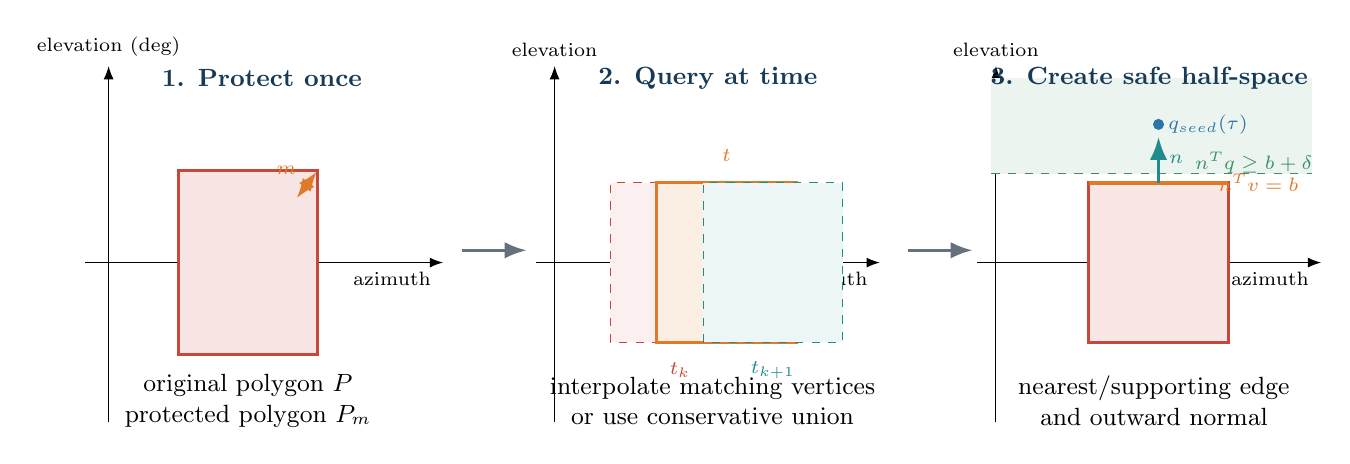
\begin{tikzpicture}[x=0.59cm,y=0.78cm,>=Latex]
% panel 1
\begin{scope}[shift={(0,0)}]
  \draw[->] (-0.5,0)--(7.2,0);
  \node[below,font=\scriptsize] at (6.1,0) {azimuth};
  \draw[->] (0,-2.6)--(0,3.2) node[above,font=\scriptsize]{elevation (deg)};
  \fill[blue!18] (2,-1) rectangle (4,1);
  \draw[blue,line width=1pt] (2,-1) rectangle (4,1);
  \fill[red!14] (1.5,-1.5) rectangle (4.5,1.5);
  \draw[red,line width=1.1pt] (1.5,-1.5) rectangle (4.5,1.5);
  \draw[<->,orange,line width=.9pt] (4.05,1.05)--(4.48,1.48)
    node[midway,above left,font=\scriptsize]{$m$};
  \node[font=\small,align=center] at (3,-2.25)
    {original polygon $P$\\protected polygon $P_m$};
  \node[font=\bfseries\small,navy] at (3.3,3.0) {1. Protect once};
\end{scope}

\draw[->,line width=1.1pt,muted] (7.6,0.2)--(9.0,0.2);

% panel 2
\begin{scope}[shift={(9.6,0)}]
  \draw[->] (-0.4,0)--(7.0,0);
  \node[below,font=\scriptsize] at (5.9,0) {azimuth};
  \draw[->] (0,-2.6)--(0,3.2) node[above,font=\scriptsize]{elevation};
  \fill[red!8] (1.2,-1.3) rectangle (4.2,1.3);
  \draw[red,dashed] (1.2,-1.3) rectangle (4.2,1.3);
  \fill[orange!13] (2.2,-1.3) rectangle (5.2,1.3);
  \draw[orange,line width=1pt] (2.2,-1.3) rectangle (5.2,1.3);
  \fill[teal!8] (3.2,-1.3) rectangle (6.2,1.3);
  \draw[teal,dashed] (3.2,-1.3) rectangle (6.2,1.3);
  \node[red,font=\scriptsize] at (2.7,-1.75) {$t_k$};
  \node[orange,font=\scriptsize] at (3.7,1.75) {$t$};
  \node[teal,font=\scriptsize] at (4.7,-1.75) {$t_{k+1}$};
  \node[font=\small,align=center] at (3.4,-2.25)
    {interpolate matching vertices\\or use conservative union};
  \node[font=\bfseries\small,navy] at (3.3,3.0) {2. Query at time};
\end{scope}

\draw[->,line width=1.1pt,muted] (17.2,0.2)--(18.6,0.2);

% panel 3
\begin{scope}[shift={(19.1,0)}]
  \draw[->] (-0.4,0)--(7.0,0);
  \node[below,font=\scriptsize] at (5.9,0) {azimuth};
  \draw[->] (0,-2.6)--(0,3.2) node[above,font=\scriptsize]{elevation};
  \fill[red!13] (2,-1.3) rectangle (5,1.3);
  \draw[red,line width=1pt] (2,-1.3) rectangle (5,1.3);
  \draw[orange,line width=1.3pt] (2,1.3)--(5,1.3);
  \fill[green!10] (-.1,1.45) rectangle (6.8,3.0);
  \draw[green,dashed] (-.1,1.45)--(6.8,1.45);
  \coordinate (s) at (3.5,2.25);
  \fill[blue] (s) circle (2pt) node[right,font=\scriptsize]{$q_{seed}(\tau)$};
  \draw[->,teal,line width=1.2pt] (3.5,1.3)--(3.5,2.05)
    node[midway,right,font=\scriptsize]{$n$};
  \node[orange,font=\scriptsize] at (5.65,1.3) {$n^Tv=b$};
  \node[green,font=\scriptsize] at (5.55,1.63) {$n^Tq\ge b+\delta$};
  \node[font=\bfseries\small,navy] at (3.3,3.0) {3. Create safe half-space};
  \node[font=\small,align=center] at (3.4,-2.25)
    {nearest/supporting edge\\and outward normal};
\end{scope}
\end{tikzpicture}
\caption{Obstacle-to-HS3 geometry transformation. Protection is already in
the polygon before HS3. At an association time, the seed chooses an exterior
side and the protected polygon becomes a local affine half-space.}
\label{fig:obstaclepipeline}
\end{figure}
\clearpage

\subsection{Seed topology before optimization}

The direct start-to-goal seed is always retained as a proposal. For obstacles,
the search layer samples source times, interval midpoints, and bounded uniform
times, then unions protected shapes into a swept planar shape. Boundary
vertices, start, and goal become visibility nodes. Candidate vertices are
offset outward by at least $10^{-3}$ degree and clipped to the workspace.
Delaunay edges provide a sparse candidate set with a bounded exhaustive
fallback; visible edges use Euclidean degree length.

The graph state is augmented with a bounded two-dimensional winding/homology
signature so distinct sampled route classes can be retained. This is an
implementation-specific planar adaptation inspired by search with homotopy
class constraints\cite{bhattacharya2012}; it is not the cited paper's full
three-dimensional construction and is not a continuous space-time homotopy
certificate.

For changing geometry, a forward time-expanded graph uses state
$(\text{time layer},\text{visibility node})$. Wait and motion edges move to a
later layer. A 13-point check filters each motion proposal, but that check is
only a search heuristic; it is never the final collision certificate.

\begin{figure}[ht]
\centering
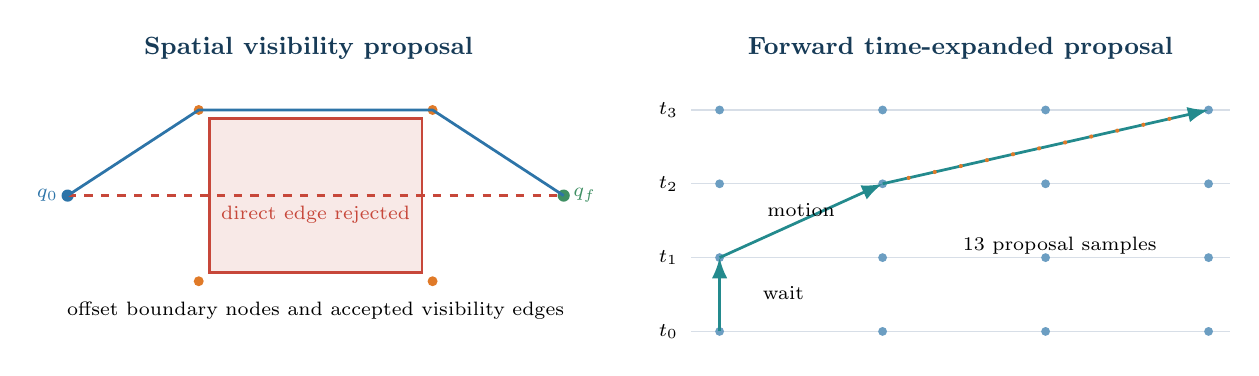
\begin{tikzpicture}[x=0.9cm,y=0.75cm,>=Latex]
\node[font=\bfseries\small,navy] at (3.4,4.8) {Spatial visibility proposal};
\fill[red!12] (2,1) rectangle (5,3.6);
\draw[red,line width=1pt] (2,1) rectangle (5,3.6);
\fill[blue] (0,2.3) circle (2.2pt) node[left,font=\scriptsize]{$q_0$};
\fill[green] (7,2.3) circle (2.2pt) node[right,font=\scriptsize]{$q_f$};
\foreach \p in {(1.85,.85),(1.85,3.75),(5.15,.85),(5.15,3.75)}
  \fill[orange] \p circle (1.8pt);
\draw[red,dashed,line width=1pt] (0,2.3)--(7,2.3)
  node[midway,below,font=\scriptsize]{direct edge rejected};
\draw[blue,line width=1pt] (0,2.3)--(1.85,3.75)--(5.15,3.75)--(7,2.3);
\node[font=\scriptsize,align=center] at (3.5,.35)
{offset boundary nodes and accepted visibility edges};

\begin{scope}[shift={(9.2,0)}]
\node[font=\bfseries\small,navy] at (3.4,4.8) {Forward time-expanded proposal};
\foreach \y/\t in {0/$t_0$,1.25/$t_1$,2.5/$t_2$,3.75/$t_3$}{
  \draw[line] (-.4,\y)--(7.2,\y);
  \node[left,font=\scriptsize] at (-.45,\y) {\t};
  \foreach \x in {0,2.3,4.6,6.9} \fill[blue!70] (\x,\y) circle (1.6pt);
}
\draw[teal,line width=1pt,->] (0,0)--(0,1.25);
\draw[teal,line width=1pt,->] (0,1.25)--(2.3,2.5);
\draw[teal,line width=1pt,->] (2.3,2.5)--(6.9,3.75);
\foreach \f in {0.08,0.16,...,0.92}
  \fill[orange] ($(2.3,2.5)!\f!(6.9,3.75)$) circle (.75pt);
\node[font=\scriptsize] at (4.8,1.45) {13 proposal samples};
\node[font=\scriptsize] at (.9,.65) {wait};
\node[font=\scriptsize] at (1.15,2.05) {motion};
\end{scope}
\end{tikzpicture}
\caption{The spatial and timed graph stages propose topology and event timing.
They do not certify the final polynomial trajectory.}
\label{fig:visibility}
\end{figure}

\subsection{Polygon side to affine HS3 row}

At dense association coordinates $\tau$, including obstacle event times, the
planner interpolates the seed and queries each protected obstacle. For selected
edge $e=B-A$, the unit left normal is

\begin{equation}
\ell=\frac{[-e_y,e_x]}{\lVert e\rVert_2}.
\end{equation}

The stored outward sign $s$ (or a probe-based sign for complex geometry) gives
$n=s\ell$. For a convex supporting plane,

\begin{equation}
b=\max_{v\in P_m(t)} n^Tv.
\end{equation}

For a selected non-supporting edge, $b=n^TA$. The required separation is
$\delta=\max(10^{-4}\ \mathrm{deg},\epsilon_{collision})$, and the optimizer
inequality is

\begin{equation}\label{eq:obstaclehalfspace}
c(\tau)=b+\delta-n^Tq(\tau)\le0,
\quad\text{equivalently}\quad n^Tq(\tau)\ge b+\delta.
\end{equation}

Stationary associations may own a complete subinterval. Projecting the HS3
position polynomial onto $n$ and converting it to Bernstein coefficients gives

\begin{equation}
c_r=b+\delta-\beta_r(n^Tq)\le0\quad\text{for every coefficient }r.
\end{equation}

\begin{figure}[ht]
\centering
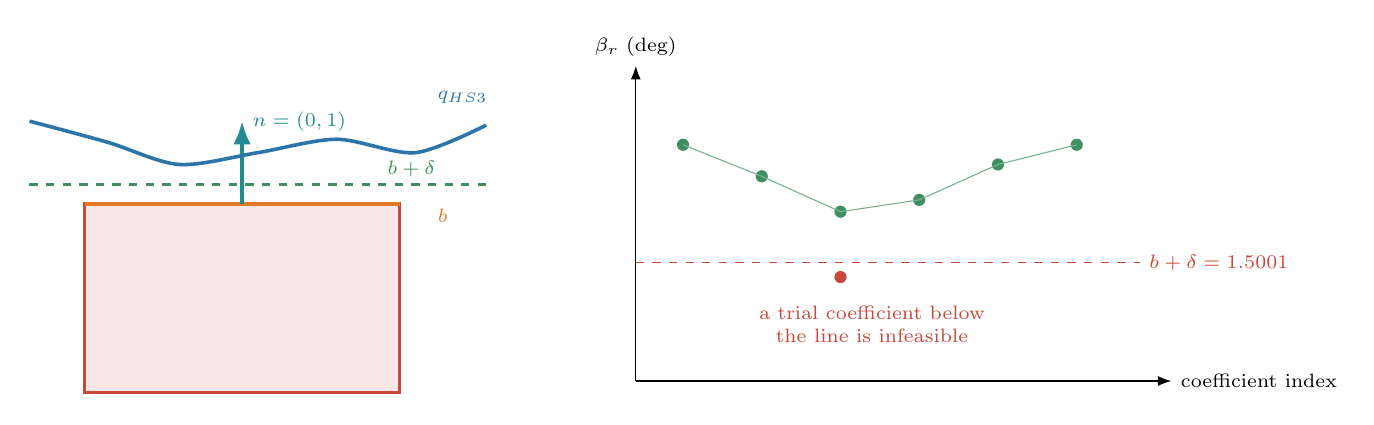
\begin{tikzpicture}[x=1cm,y=1cm,>=Latex]
\begin{scope}
  \fill[red!13] (1,0) rectangle (5,2.4);
  \draw[red,line width=1pt] (1,0) rectangle (5,2.4);
  \draw[orange,line width=1.4pt] (1,2.4)--(5,2.4);
  \draw[green,dashed,line width=1pt] (.3,2.65)--(6.2,2.65);
  \draw[->,teal,line width=1.2pt] (3,2.4)--(3,3.45)
    node[right,font=\scriptsize]{$n=(0,1)$};
  \draw[blue,line width=1.3pt]
    plot[smooth] coordinates {(.3,3.45) (1.3,3.18) (2.2,2.9)
      (3.2,3.05) (4.2,3.22) (5.2,3.05) (6.1,3.4)};
  \node[blue,font=\scriptsize] at (5.8,3.75) {$q_{HS3}$};
  \node[green,font=\scriptsize] at (5.15,2.84) {$b+\delta$};
  \node[orange,font=\scriptsize] at (5.55,2.25) {$b$};
\end{scope}
\begin{scope}[shift={(8.0,.15)}]
  \draw[->] (0,0)--(6.8,0) node[right,font=\scriptsize]{coefficient index};
  \draw[->] (0,0)--(0,4.0) node[above,font=\scriptsize]{$\beta_r$ (deg)};
  \draw[red,dashed] (0,1.5)--(6.4,1.5)
    node[right,font=\scriptsize]{$b+\delta=1.5001$};
  \foreach \x/\y in {0.6/3.0,1.6/2.6,2.6/2.15,3.6/2.3,4.6/2.75,5.6/3.0}
    \fill[green] (\x,\y) circle (2.2pt);
  \draw[green!70] plot coordinates {(.6,3.0) (1.6,2.6) (2.6,2.15)
    (3.6,2.3) (4.6,2.75) (5.6,3.0)};
  \fill[red] (2.6,1.32) circle (2.2pt);
  \node[red,font=\scriptsize,align=center] at (3.0,.72)
    {a trial coefficient below\\the line is infeasible};
\end{scope}
\end{tikzpicture}
\caption{A stationary obstacle support becomes a complete-interval Bernstein
constraint. Every green coefficient above the threshold certifies the entire
projected polynomial span.}
\label{fig:bernsteinhalfspace}
\end{figure}

\subsection{Moving obstacles and the authority of validation}

Moving/deforming geometry uses ordered frozen-time associations during the
local solve. A fast-moving association can be locked while the seed continues
to satisfy it. These rows guide the optimizer but are not treated as a complete
continuous collision proof.

Independent validation splits every HS3 segment at obstacle source times,
checks endpoints, and adaptively bisects intervals. If midpoint clearance is
$d_m$, the conservative relative-motion allowance for interval width
$\Delta t$ is

\begin{equation}\label{eq:collisioncertificate}
r=\left(\lVert v_{path,max}\rVert_2+v_{obs,max}\right)
\frac{\Delta t}{2}.
\end{equation}

The interval is certified only when
$d_m>r+\epsilon_{collision}$. Otherwise it is bisected. If the minimum allowed
time step is reached without proof, validation fails; it never silently
accepts an unresolved interval.

\begin{figure}[ht]
\centering
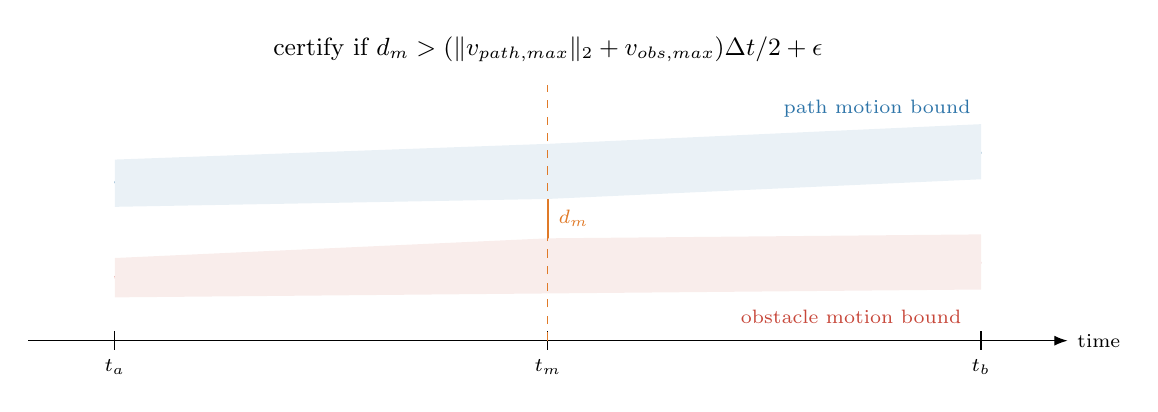
\begin{tikzpicture}[x=1.1cm,y=1cm,>=Latex]
  \draw[->] (0,0)--(12,0) node[right,font=\scriptsize]{time};
  \foreach \x/\lab in {1/$t_a$,6/$t_m$,11/$t_b$}{
    \draw (\x,.12)--(\x,-.12) node[below,font=\scriptsize]{\lab};
  }
  \draw[blue,line width=1.2pt] (1,2.0)..controls (4,3.0) and (8,1.2)..(11,2.4);
  \draw[red,line width=1.2pt] (1,.8)..controls (4,1.35) and (8,.55)..(11,1.0);
  \fill[blue] (6,2.15) circle (2pt);
  \fill[red] (6,.95) circle (2pt);
  \draw[<->,orange,line width=1pt] (6,1.0)--(6,2.1)
    node[midway,right,font=\scriptsize]{$d_m$};
  \fill[blue!10] (1,1.7)--(1,2.3)--(6,2.5)--(11,2.75)--(11,2.05)--(6,1.8)--cycle;
  \fill[red!10] (1,.55)--(1,1.05)--(6,1.3)--(11,1.35)--(11,.65)--(6,.6)--cycle;
  \node[blue,font=\scriptsize] at (9.8,2.95) {path motion bound};
  \node[red,font=\scriptsize] at (9.5,.3) {obstacle motion bound};
  \node[font=\small,align=center] at (6,3.7)
    {certify if $d_m>(\lVert v_{path,max}\rVert_2+v_{obs,max})\Delta t/2+\epsilon$};
  \draw[orange,dashed] (6,0)--(6,3.25);
\end{tikzpicture}
\caption{Adaptive collision certificate. Failure to establish separation
causes bisection; an unresolved minimum-size interval is a validation failure.}
\label{fig:adaptivevalidation}
\end{figure}

\subsection{Azimuth wrapping limitation}

This commit does not wrap or seam-replicate obstacles. When any obstacle is
present, \file{AllowAzimuthWrapping=true} is rejected. Obstacle-free fixed-goal
requests may shift the goal azimuth by an integer multiple of 360 degrees to
select the nearest equivalent representation. Graphics must therefore not be
read as a periodic obstacle transformation.

\section{Solver, candidate, and result logic}

\subsection{Warm start from a topology seed}

A route seed is parameterized by cumulative planar arc length to obtain
$q_{seed}(\tau)$. The solver samples it at the HS3 control coordinates and
fits jerk ordinates by regularized least squares using exact affine sensitivity
maps. Desired velocity follows local route tangents, is bounded by axis limits,
and respects endpoint derivatives. The fitted jerk is clipped to the configured
limit and used only as an initialization; it does not define reachability.

\subsection{Fixed and free solve paths}

\begin{longtable}{@{}p{.19\linewidth}p{.38\linewidth}p{.37\linewidth}@{}}
\toprule
Property & Fixed arrival & Earliest arrival \\
\midrule
\endhead
Decision & $J$ & $J$ and $t_f$ \\
Objective & Integrated squared jerk, Equation~\eqref{eq:jerkcost} & Absolute final time \\
Constraint structure & Affine in jerk after corridor association & Nonlinear because duration changes maps and geometry time \\
Primary numerical method & Convex QP through \file{quadprog} & Local NLP through \file{fmincon} \\
Derivative policy & Exact matrices and exact objective gradient/Hessian & Exact jerk columns; safeguarded final-time difference \\
Candidate ranking & Shortest validated sampled motion, then jerk & Earliest within arrival tolerance, then jerk \\
\bottomrule
\end{longtable}

\subsection{Mesh refinement and corridor relinearization}

The planner can retry a candidate with updated obstacle associations and can
increase the segment count within configured work limits. These are bounded
attempts. They do not imply convergence, completeness, or discovery of every
homotopy class. Diagnostics retain every attempted seed, mesh, relinearization,
solver state, validation state, and relevant rejection count.

\subsection{Independent acceptance rule}

An optimizer-feasible result is only a candidate. Public acceptance requires
the independent validator to pass:

\begin{itemize}
  \item stable finite histories and a strictly increasing time base;
  \item exact initial and terminal position/velocity/acceleration agreement;
  \item workspace and full continuous position/velocity/acceleration/jerk
  bounds from the returned polynomial;
  \item continuous collision clearance against protected geometry across
  obstacle time history;
  \item safety-margin and coordinate-wrap policy consistency;
  \item a valid static seed-corridor certificate where applicable.
\end{itemize}

The returned \file{Success} becomes true only after this validation. Constraint
violations are reported; the trajectory is not clipped to hide them.

\section{Simple rectangle walkthrough}\label{sec:walkthrough}

This section uses small hand-calculated values to show the data transformation.
It is an explanatory trace, not recorded optimizer output.

\subsection{Step 1: define the physical request}

Let the original static obstacle be

\begin{equation}
P=[4,6]\times[-1,1]\ \mathrm{deg},\qquad t=[0]\ \mathrm{s},
\end{equation}

with safety margin $m=0.5$ degree. Let

\begin{align*}
q_0&=(0,0)\ \mathrm{deg}, & t_0&=0\ \mathrm{s},\\
q_f&=(10,0)\ \mathrm{deg},& t_f&=12\ \mathrm{s},
\end{align*}

and use zero endpoint velocity/acceleration, velocity limit
$(2,2)$ deg/s, acceleration limit $(1,1)$ deg/s$^2$, and jerk limit
$(2,2)$ deg/s$^3$.

\subsection{Step 2: apply the margin once}

The square-joint buffer produces the protected rectangle

\begin{equation}
P_m=[3.5,6.5]\times[-1.5,1.5]\ \mathrm{deg}.
\end{equation}

Both the original and protected coordinates remain in the obstacle record.
Every downstream search, corridor, occupancy, and collision operation uses
$P_m$; it does not add another 0.5 degree.

\subsection{Step 3: detect that the direct seed is blocked}

The direct spatial seed is $q(\tau)=(10\tau,0)$. It intersects $P_m$ for
$\tau\in[0.35,0.65]$. The direct seed remains in diagnostics as a proposal, but
it cannot pass collision validation.

\subsection{Step 4: create a detour topology}

The protected swept shape equals $P_m$ because the obstacle is static. A
visibility route can pass above or below. For arithmetic, take the conceptual
top seed

\begin{equation}
(0,0)\rightarrow(3.5,2.0)\rightarrow(6.5,2.0)\rightarrow(10,0).
\end{equation}

The actual graph offsets boundary vertices by at least 0.001 degree; exact
vertex order depends on MATLAB's polygon boundary traversal. The route is
parameterized by cumulative arc length, producing $q_{seed}(\tau)$.

\subsection{Step 5: create HS3 decisions}

With the default $N=10$ segments, each axis has $2N+1=21$ jerk ordinates.
The fixed-time decision therefore has 42 values. Earliest arrival would append
one final-time value. The warm-start fit uses the seed at control coordinates,
but the optimizer is free to move the trajectory while satisfying its
constraints.

\subsection{Step 6: turn the top obstacle edge into a row}

At a seed point near $(5,2)$, the nearest protected edge is the top edge
$y=1.5$. Its outward normal and support are

\begin{equation}
n=(0,1),\qquad b=1.5\ \mathrm{deg}.
\end{equation}

With $\delta=10^{-4}$ degree, Equation~\eqref{eq:obstaclehalfspace} becomes

\begin{equation}
[0\ \ 1]q(\tau)\ge1.5001,
\quad\text{or}\quad 1.5001-\mathrm{elevation}(\tau)\le0.
\end{equation}

Suppose the projected quintic position on the associated segment has
Bernstein coefficients

\begin{equation}
[2.00,1.80,1.65,1.70,1.90,2.00]\ \mathrm{deg}.
\end{equation}

Every coefficient exceeds 1.5001 degree, so the complete segment is certified
above that support. A trial coefficient of 1.49 degree would violate the row by
0.0101 degree and be infeasible.

\subsection{Step 7: optimize and reconstruct}

For the fixed 12-second request, the solver minimizes integrated squared jerk
subject to endpoint state, continuous kinematic, topology corridor, and
obstacle support constraints. Equation~\eqref{eq:jerk} is integrated exactly
to reconstruct position, velocity, acceleration, and jerk histories. Sampled
output contains uniform points plus every polynomial knot.

\subsection{Step 8: independently validate and select}

The public validator rechecks the returned polynomial, derivative bounds, and
protected polygon clearance. A top and bottom route may both validate. Fixed
arrival selects the shortest validated sampled motion, breaking ties with
integrated squared jerk. If none validates, the planner returns
\file{Success=false}, \file{TerminationReason="noValidatedSeed"}, and preserves
the best partial candidate and search diagnostics.

\subsection{Moving extension}

If the same original rectangle translates 2 degrees in azimuth between
$t=0$ and $t=10$ seconds, the protected vertices translate identically. At
$t=5$ seconds, $\lambda=0.5$ and

\begin{equation}
P_m(5)=[4.5,7.5]\times[-1.5,1.5],\qquad v_{obs,max}=0.2\ \mathrm{deg/s}.
\end{equation}

For a validation interval $\Delta t=0.1$ second and path speed bound
$\lVert v_{path,max}\rVert_2=2$ deg/s, Equation~\eqref{eq:collisioncertificate}
gives $r=(2+0.2)(0.05)=0.11$ degree. Midpoint clearance must exceed
$0.11+\epsilon_{collision}$ or the interval is bisected.

\section{Defaults, diagnostics, and failure behavior}

\subsection{Obstacle-planner defaults at the documented commit}

\begin{longtable}{@{}p{.36\linewidth}p{.22\linewidth}p{.34\linewidth}@{}}
\toprule
Option & Default & Meaning \\
\midrule
\endhead
\file{GoalTimeMode} & \file{earliestArrival} & Minimize arrival within the supplied horizon. \\
\file{SampleTime_s} & 0.05 & Returned uniform sampling interval; knots are also retained. \\
\file{AllowAzimuthWrapping} & false & Periodic goal representation is disabled by default. \\
\file{MaximumSeedCount} & 5 & Bounded topology proposal count. \\
\file{DirectOnly} & false & Permit visibility, homology, and timed seeds. \\
\file{ObstacleClusterDistance_deg} & 0 & Disable nearby-region seed clustering. \\
\file{CollocationSegmentCount} & 10 & Initial equal-duration HS3 segment count. \\
\file{MaximumCollocationSegmentCount} & 64 & Mesh-refinement cap. \\
\file{MaximumMeshRefinementPasses} & 2 & Bounded refinement attempts. \\
\file{MaximumNlpIterations} & 300 & Local solver iteration cap. \\
\file{MaximumFunctionEvaluations} & 30000 & Solver evaluation cap. \\
\file{MaximumPlanningTime_s} & 115 & Cooperative outer planning budget. \\
\file{DeterministicWorkBudget} & false & Wall-time budget remains active by default. \\
\file{ArrivalTimeTolerance_s} & $10^{-3}$ & Arrival comparison/refinement tolerance. \\
\file{ConstraintTolerance} & $10^{-7}$ & Numerical constraint tolerance. \\
\file{OptimalityTolerance} & $10^{-7}$ & Local solver optimality tolerance. \\
\file{StepTolerance} & $10^{-10}$ & Local solver step tolerance. \\
\file{CollisionClearanceTolerance_deg} & $10^{-7}$ & Clearance tolerance for validation. \\
\file{CollisionMinimumTimeStep_s} & 0.00025 & Fail-closed adaptive collision resolution floor. \\
\file{RandomSeed} & 0 & Echoed deterministic seed; search is deterministic. \\
\bottomrule
\end{longtable}

The neutral \file{solveTrajHS3} defaults use generic names and a narrower scope:
earliest arrival, $N=10$, sample time 0.05, 300 iterations, 30,000 evaluations,
115 time units of solve budget, $10^{-3}$ arrival tolerance, $10^{-7}$
constraint/optimality tolerances, $10^{-10}$ step tolerance, and quiet output.

\subsection{First-class diagnostics}

Search diagnostics are collected while searching. They include nodes, accepted
and rejected edges, time layers, parent/cost relationships, homology/timed
coverage, work-limit evidence, seed provenance, and the best partial state.
Candidate summaries retain optimizer status, maximum violation, collision
resolution, clearance, mesh/relinearization counts, timing, and solver output.
Seven exclusive stage-timing fields reconcile to an independently measured
total.

\subsection{Expected failures}

Recognized expected outcomes include endpoint infeasibility, exact static
no-route/no validated seed, time-window infeasibility, local optimizer
infeasibility, solver time limit, arrival pinned to the horizon, and validation
failure. The standalone engine additionally reports an infeasible time horizon.
All use stable output schemas. Invalid dimensions, missing fields, malformed
histories, unsupported wrapping, unknown planner method, or corrupt internal
state use identified errors.

\section{Known limitations and interpretation}\label{sec:limits}

\begin{itemize}
  \item The deterministic topology portfolio is finite and is not complete.
  A returned no-path result means no configured proposal produced an
  independently valid motion; it is not a mathematical proof that no motion
  exists unless the exact static graph condition specifically applies.
  \item Earliest-arrival HS3 is a local nonlinear method. It does not prove
  global minimum arrival or global optimality.
  \item Static earliest-arrival planning may stop after the first independently
  validated seed to protect the time budget, so an unattempted topology may be
  faster.
  \item Arrival quality is mesh-limited. A coarse mesh may yield a later valid
  arrival; refinement costs more solver work.
  \item Moving/deforming obstacle rows are local frozen-time associations.
  Independent adaptive polygon validation is authoritative between those
  association times.
  \item Azimuth wrapping with obstacles or moving goals is unsupported.
  \item One solver evaluation or callback may finish after the cooperative
  time limit, so measured elapsed time can overrun the nominal budget.
  \item Geographic and Az/El geometry is planar in degrees, not spherical.
\end{itemize}

\section{Complete tracked MATLAB file catalog}\label{sec:inventory}

This catalog covers all 93 tracked \file{.m} files at the documented commit.
"Called by" descriptions identify principal ownership, not every test call.

\subsection{Production: geometry}

\scriptentry{+obstacleAvoidance/+geometry/boundaryToEdges.m}{Converts every
connected \file{polyshape} boundary ring into deterministic N-by-2 start/end
edge rows. It removes only an explicitly repeated closing vertex and then
closes each valid ring. Clearance and visibility code use it to enumerate
actual polygon segments.}

\scriptentry{+obstacleAvoidance/+geometry/boundaryToShape.m}{Converts paired,
NaN-separated azimuth/elevation vectors to an unsimplified \file{polyshape}.
It preserves ring correspondence and collinear vertices; fewer than three
finite vertices yields empty geometry. Dynamic preparation, time queries, and
corridor construction depend on this canonical conversion.}

\scriptentry{+obstacleAvoidance/+geometry/canonicalBoundaryToEdges.m}{Turns a
canonical geometry record into directed closed edges in source order. Moving
obstacle association and constraint evaluation use the stable ordering to keep
edge identity and outward direction reproducible.}

\scriptentry{+obstacleAvoidance/+geometry/convexPolygonRegions.m}{Decomposes
occupied polygon geometry into convex regions. Already-convex regions are kept;
nonconvex components are triangulated. Seed-corridor and corridor-certificate
logic require convex components so one supporting half-space has valid local
meaning.}

\scriptentry{+obstacleAvoidance/+geometry/pointPolygonClearance.m}{Computes
signed Euclidean clearance, nearest boundary point, and deterministic edge
index for N-by-2 query points. Positive is outside, negative is inside, and an
empty shape gives infinity. Occupancy, clustering, corridors, validation, and
tests share this implementation.}

\subsection{Production: input normalization}

\scriptentry{+obstacleAvoidance/+input/goalPositionAtTime.m}{Evaluates either a
fixed goal or an interpolated sampled moving goal at absolute times. Endpoint
checks, route search, terminal constraints, intercept planning, validation, and
plotting call it so target interpretation stays consistent.}

\scriptentry{+obstacleAvoidance/+input/normalizeLogicalScalar.m}{Implements the
repository-wide scalar logical or binary-numeric contract while preserving the
owning caller's error identifier and field name. Options, plotting, obstacle,
example, intercept, and sandbox controls reuse it.}

\scriptentry{+obstacleAvoidance/+input/normalizePlannerRequest.m}{Canonicalizes
the public obstacle/state/limit request. It combines obstacles, converts numeric
orientations to 1-by-2 doubles, defaults endpoint derivatives, supplies
workspace intervals, checks cross-field dimensions, and implements the limited
obstacle-free azimuth-wrap policy.}

\scriptentry{+obstacleAvoidance/+input/resolveHs3Options.m}{Owns and validates
all obstacle-aware HS3 defaults. Partial or empty overrides are merged through
the shared resolver; unknown fields warn once and do not affect behavior. It
also emits migration errors for fields whose ownership changed.}

\scriptentry{+obstacleAvoidance/+input/resolveOptions.m}{A generic partial
scalar-structure merge. It retains default field order, substitutes defaults
for omitted/empty values, returns unknown names without applying them, and is
used by public options owners and display/query helpers.}

\scriptentry{+obstacleAvoidance/+input/validatePlannerEndpoints.m}{Performs the
pre-search feasibility screen: start/goal occupancy, workspace bounds,
derivative limits, time ordering, and goal-time policy. It returns an expected
failure reason/message instead of throwing for a physically infeasible request.}

\subsection{Production: obstacle infrastructure}

\scriptentry{+obstacleAvoidance/+obstacles/combineObstacles.m}{Flattens obstacle
arrays, nested cells, and empty inputs into one canonical column array while
preserving caller order. It delegates normalization to \file{createObstacle}
and provides a schema-preserving empty array.}

\scriptentry{+obstacleAvoidance/+obstacles/createMovingObstacle.m}{Evaluates a
caller transform independently at every increasing source time and constructs
one canonical moving/deforming obstacle plus history metrics. It assumes no
rigid motion, shared vertex count, or shared topology.}

\scriptentry{+obstacleAvoidance/+obstacles/createObstacle.m}{The sole public
obstacle constructor, normalizer, and protection rebuilder. It validates
NaN-separated rings, preserves original/protected histories, applies an
absolute square-joint \file{polybuffer} margin once, reuses exact translated
protection when possible, and returns the stable canonical schema.}

\scriptentry{+obstacleAvoidance/+obstacles/hasChangingHistory.m}{Classifies
whether obstacle geometry or activation span changes over the requested plan.
Search uses this result to decide whether a time-expanded topology proposal is
needed.}

\scriptentry{+obstacleAvoidance/+obstacles/prepareDynamic.m}{Precomputes sample
shapes, history bounds, interval unions, interpolation deltas, topology flags,
and vertex speed bounds. Matching topology is interpolated vertexwise;
topology-changing intervals use a conservative stationary union.}

\scriptentry{+obstacleAvoidance/+obstacles/queryObstacleOccupancyAtTime.m}{The
public point/time occupancy and signed-clearance query. It broadcasts compatible
inputs, uses prepared broad-phase bounds, queries already-protected shapes,
reports the first blocker and detailed provenance, and treats the boundary as
occupied by default.}

\scriptentry{+obstacleAvoidance/+obstacles/shapeAtTime.m}{Returns the active
protected shape and metadata at one physical time. It reuses exact source
slices, interpolates matching vertices, returns conservative unions for
topology changes, and reports convexity, outward sign, and speed information
used by corridor construction.}

\subsection{Production: planner}

\scriptentry{+obstacleAvoidance/+planner/createConstraintMatrices.m}{Builds the
exact fixed-duration HS3 inequality/equality Jacobians in solver row order. It
combines continuous Bernstein bounds, terminal P/V/A equations, static seed
corridors, frozen obstacle corridors, and optional direct-line collinearity
equations through the affine sensitivity model.}

\scriptentry{+obstacleAvoidance/+planner/createEmptyResult.m}{Creates the single
stable obstacle-planner result, seed-summary, polynomial, validation, and search
diagnostic templates. Every success and failure exit inherits identical field
order and explicit empty values.}

\scriptentry{+obstacleAvoidance/+planner/createEmptySolverDiagnostics.m}{Creates
and finalizes the stable solver diagnostic schema, including distinct solver
and outer elapsed times. Candidate construction uses it even when no numerical
solve ran.}

\scriptentry{+obstacleAvoidance/+planner/evaluatePlannerPolynomial.m}{Adapts the
unit-bearing obstacle-planner polynomial record to the dimension-neutral
polynomial evaluator and returns absolute time plus position, velocity,
acceleration, and jerk histories.}

\scriptentry{+obstacleAvoidance/+planner/evaluateTrajectoryConstraints.m}{Evaluates
all planner inequalities/equalities and gradients. It adds continuous
Bernstein kinematic bounds, seed/topology corridors, time-indexed obstacle
associations, terminal state, exact jerk Jacobian columns, and a safeguarded
variable-final-time column.}

\scriptentry{+obstacleAvoidance/+planner/plan.m}{The maintained internal
orchestrator. It resolves and normalizes, validates endpoints, prepares dynamic
geometry, creates deterministic seeds, manages budgets, solves/relinearizes/
refines candidates, independently validates them, ranks valid outcomes, and
assembles a stable success or evidence-rich failure.}

\scriptentry{+obstacleAvoidance/+planner/solveRouteCandidate.m}{Transforms one
route seed into an HS3 problem. It sets mesh/control layout, fits a bounded jerk
warm start, creates topology and moving-obstacle corridor associations, invokes
the neutral solver executor, reconstructs exact polynomials, samples the motion,
and returns one stable candidate and solver diagnostics.}

\scriptentry{+obstacleAvoidance/+planner/stageTiming.m}{Defines and reconciles
the seven exclusive planner timing fields against an independently measured
total. It rejects over-attribution and applies the finalized timing schema at
the public boundary.}

\scriptentry{+obstacleAvoidance/+planner/validatePolynomialTrajectory.m}{Checks
the returned polynomial schema, time basis, continuity, endpoint state,
sampled histories, and complete continuous coordinate/derivative bounds. It
uses polynomial coefficients rather than trusting samples alone.}

\subsection{Production: search and certification}

\scriptentry{+obstacleAvoidance/+search/boundedTimeLayers.m}{Combines source-aware
and uniformly spaced time layers, retains endpoints, and applies a deterministic
cap. Route generation and the time-expanded search use it to bound work without
discarding event provenance silently.}

\scriptentry{+obstacleAvoidance/+search/certifySeedCorridor.m}{Independently
verifies a solver-supplied static corridor certificate. It checks schema,
complete obstacle-envelope containment, supporting half-spaces, and the entire
returned polynomial through Bernstein inequalities; uncertainty fails closed.}

\scriptentry{+obstacleAvoidance/+search/createRouteCandidates.m}{Creates the
bounded deterministic route portfolio and first-class search diagnostics. It
retains the direct proposal, builds swept geometry and visibility nodes/edges,
adds a timed route for changing history, enumerates distinct homology classes,
and only shortens a route when visibility and signature are preserved.}

\scriptentry{+obstacleAvoidance/+search/createSeedCorridor.m}{Converts convex
seed-envelope regions to per-segment exterior support records. A seed midpoint
chooses the free side and a retained clearance; later certification verifies
the complete polynomial rather than trusting that midpoint.}

\scriptentry{+obstacleAvoidance/+search/denseSweptEnvelope.m}{Replaces an
unaffordable exact swept union with a conservative directional-support hull for
seed generation. It protects source endpoints, clips against support planes,
and reports whether the approximation was used.}

\scriptentry{+obstacleAvoidance/+search/seedCorridorInequality.m}{Projects each
position polynomial onto its seed-corridor normal, converts to Bernstein form,
and emits finite inequalities that enforce continuous exterior separation over
the complete segment.}

\scriptentry{+obstacleAvoidance/+search/seedEnvelopeContainsObstacles.m}{Checks
that one connected corridor boundary contains a conservative continuous sweep
of every protected obstacle. Incomplete containment prevents a static corridor
from being treated as a certificate.}

\scriptentry{+obstacleAvoidance/+search/timeExpandedVisibilitySearch.m}{Searches
a forward layered graph whose state is time layer plus visibility node. It
supports waiting and motion arcs, uses bounded sampled collision filtering, and
returns route positions, absolute route times, parents, costs, and work counts.}

\subsection{Production: public APIs and plotting}

\scriptentry{+obstacleAvoidance/planMovingTargetIntercept.m}{Adapts a sampled
target history to the maintained public trajectory planner. Specified-time mode
runs one plan; earliest mode performs bounded chronological trials and refines
only the first observed feasible bracket. Target derivatives are derived
consistently from the sampled track.}

\scriptentry{+obstacleAvoidance/planTrajectory.m}{The public HS3-only planner
entry point and zero-input/defaults query. It validates the sole supported
\file{PlannerMethod="hs3"}, removes the selector, and dispatches to the
internal orchestrator under the stable public contract.}

\scriptentry{+obstacleAvoidance/validateTrajectory.m}{The independent public
validator. It combines polynomial/endpoint/continuous-bound checks with
adaptive protected-polygon collision certification, safety-margin and wrap
policy checks, and optional static corridor certification. Unresolved intervals
fail rather than pass by sampling.}

\scriptentry{+obstacleAvoidance/+plotting/plotTrajectory.m}{Creates spatial
search/motion, animation, and position/velocity/acceleration/jerk views solely
from the returned result. It distinguishes original/protected geometry and
accepted/rejected search evidence, respects figure/animation controls, and
never reruns planning.}

\subsection{Dimension-neutral HS3 engine}

\scriptentry{hs3/solveTrajHS3.m}{The public D-dimensional fixed-time or
earliest-arrival boundary-value solver. It owns the generic input contract,
normalizes optional affine point/interval path rows, calls the fixed/free
solvers, reconstructs and samples the polynomial, computes jerk cost, validates
independently, and returns one stable schema.}

\scriptentry{hs3/+hs3Internal/defaultOptions.m}{The single source of
argument-independent neutral HS3 defaults for mode, mesh, sampling, iteration,
evaluation, time, and numerical tolerances.}

\scriptentry{hs3/+hs3Internal/validate.m}{Independently checks neutral result
histories, strictly increasing time, initial/terminal P/V/A agreement, and
complete continuous/path constraints by reevaluating the returned control
decision.}

\scriptentry{hs3/+hs3Internal/+solver/optimize.m}{Executes normalized numerical
problems and produces a stable stage record. Fixed-time exact convex problems
use \file{quadprog}; free-time problems use gradient-enabled \file{fmincon}; a
bounded feasibility-recovery solve may follow. It centralizes exit flags,
violations, time limit, and error capture.}

\scriptentry{hs3/+hs3Internal/+solver/solveFixedTime.m}{Builds the fixed-duration
minimum-integrated-squared-jerk QP: exact constraint values/matrices, exact jerk
Hessian, bounds, and a minimum-norm equality-feasible initial decision. It then
delegates numerical execution to \file{optimize}.}

\scriptentry{hs3/+hs3Internal/+solver/solveFreeTime.m}{Builds the
variable-final-time arrival NLP. It first obtains a deterministic fixed-horizon
jerk seed, appends final time and its bounds, defines the exact arrival
objective, and delegates the local solve/recovery to \file{optimize}.}

\scriptentry{hs3/+hs3Internal/+constraints/createFixedConstraintMatrices.m}{Builds
exact dimension-neutral jerk Jacobians for continuous coordinate and derivative
bounds, terminal P/V/A, and optional affine point/subinterval path constraints.
Each coordinate occupies its own control block.}

\scriptentry{hs3/+hs3Internal/+constraints/evaluateConstraints.m}{Reconstructs
the decision and returns inequalities $c\le0$, equalities $c_{eq}=0$, and
\file{fmincon}-oriented gradients. Fixed-time jerk columns are exact; the
free-time column uses a bounded one-sided difference with valid room.}

\scriptentry{hs3/+hs3Internal/+polynomial/convertPowerToBernstein.m}{Converts
ascending power coefficients to same-degree Bernstein coefficients on
$[0,1]$ through a cached exact Pascal-based matrix. Continuous-bound and
corridor logic in both products use it.}

\scriptentry{hs3/+hs3Internal/+polynomial/createAffineSensitivityModel.m}{Builds
exact maps from scalar-coordinate jerk ordinates to segment polynomial
coefficients, terminal P/V/A, and requested global-$\tau$ evaluations. These
maps explain the fixed-time affine constraint structure.}

\scriptentry{hs3/+hs3Internal/+polynomial/createSubintervalBernsteinMap.m}{Maps a
normalized point/subinterval to its owning segment and creates an exact
restricted power-to-Bernstein hull map. It validates that a constraint interval
does not cross a segment boundary.}

\scriptentry{hs3/+hs3Internal/+polynomial/createTrajectoryPolynomial.m}{Exactly
integrates start/mid/end quadratic jerk across equal segments, propagating
state continuity and returning quintic position, quartic velocity, cubic
acceleration, quadratic jerk, segment times, and terminal state.}

\scriptentry{hs3/+hs3Internal/+polynomial/evaluateIntegratedSquaredJerk.m}{Computes
the exact integrated squared-jerk objective, decision gradient, and fixed-time
Hessian. The free-time gradient includes the duration dependence; a constant
Hessian is intentionally available only for fixed time.}

\scriptentry{hs3/+hs3Internal/+polynomial/evaluateTrajectoryPolynomial.m}{Evaluates
ascending-power segment records at absolute times, automatically selects the
owning segment or accepts explicit indices, clamps local coordinates to
$[0,1]$, and returns N-by-D histories.}

\subsection{Benchmarks}

\scriptentry{benchmarks/benchmarkRandomMovingPolygonStress.m}{Runs a deterministic
stress sweep of large rotating/translating/deforming polygons. It preserves the
exact request, planner result, independent validation, analytic boundary
witness, seed, and per-case diagnostics rather than regenerating failed cases.}

\scriptentry{benchmarks/benchmarkStandaloneHs3Scaling.m}{Measures repeated-turn
and hairpin scaling serially. It builds shared scenarios, enforces HS3 result
contracts, validates, and records route, solver, search, runtime, and environment
evidence for each repeat and scale.}

\scriptentry{benchmarks/compareHs3ExtractionBaseline.m}{Compares the current
neutral HS3 extraction with a frozen historical baseline. It runs candidate
reports, checks nested exact/numeric fields, reconstructs controls from
polynomials, and compares serial runtime medians without rewriting the planner.}

\scriptentry{benchmarks/createRepeatedTurnBenchmarkScenario.m}{Constructs one
scale-controlled alternating-barrier request shared by scaling work. Turn count
and options determine canonical obstacles, endpoints, limits, and documented
constants; planner logic remains scenario-independent.}

\subsection{Maintained examples and helpers}

Every scenario below follows the maintained pattern: resolve controls, create
canonical obstacles and request data, call the public planner or intercept
wrapper, validate independently, and plot the returned result when enabled.
Several deterministic moving-scene inputs use the quintic smootherstep blend
$10u^3-15u^4+6u^5$, associated with Perlin's improved-noise construction
\cite{perlin2002}. In this repository it is scenario input construction, not an
HS3 motion model.

\scriptentry{examples/exampleAlternatingSlalom.m}{Demonstrates an input-driven
route through alternating static barriers from $[-8,0]$ to $[8,0]$, exercising
multiple turns without hidden waypoints.}

\scriptentry{examples/exampleDenseConcaveObstacle.m}{Demonstrates protected
dense concave geometry and visibility-based topology selection without
scenario-specific planner guidance.}

\scriptentry{examples/exampleFortyMovingCircleGrid.m}{Plans earliest diagonal
motion through an 8-by-5 grid of 40 circles moving vertically, stressing timed
visibility, moving associations, and independent validation.}

\scriptentry{examples/exampleFourAcceleratingCircles.m}{Uses four vertically
accelerating circles and a moving target to demonstrate interception through an
early center-line opening.}

\scriptentry{examples/exampleInterceptMovingTargetAtSetTime.m}{Runs an
obstacle-free position-only intercept of a curved sampled target at a specified
time and validates the wrapper's terminal target interpretation.}

\scriptentry{examples/exampleInterceptMovingTargetEarliest.m}{Uses the public
intercept wrapper to find the earliest observed feasible obstacle-free intercept
within its bounded chronological search.}

\scriptentry{examples/exampleMovingBarrierWait.m}{Demonstrates a trajectory
that waits continuously for a translating barrier, exercising timed seeds and
nonzero event timing rather than a spatial detour alone.}

\scriptentry{examples/exampleMovingCircleNoAzimuthWrap.m}{Demonstrates an
immediate detour around a rising circle with periodic azimuth explicitly
disabled, protecting the non-wrapped obstacle contract.}

\scriptentry{examples/exampleMovingDeformingUSOutlineVisibility.m}{Creates a
dense U.S. outline that grows, deforms, rotates 180 degrees, and disappears,
with a second moving sun obstacle. It exercises changing topology/visibility and
the geographic helper.}

\scriptentry{examples/exampleNoPath.m}{Constructs a full-height wall and
expects a stable \file{noValidatedSeed} result. It independently validates the
failure record and demonstrates workspace plus time-expanded diagnostics when
plotting is enabled.}

\scriptentry{examples/exampleObstacleAvoidance.m}{The compact deterministic
one-rectangle example, demonstrating automatic side choice, protected geometry,
HS3 motion, validation, and result-driven plotting.}

\scriptentry{examples/exampleObstacleFree.m}{Exercises earliest-arrival
rest-to-rest HS3 motion without geometry, isolating kinematic bounds, arrival
optimization, and polynomial validation.}

\scriptentry{examples/exampleOpeningUShapedObstacle.m}{Waits for a U-shaped
obstacle opening and adds a scenario-local post-validation that the timed
opening, rather than an unintended route, was used.}

\scriptentry{examples/exampleStaticUShapedObstacle.m}{Demonstrates escape from
a protected static U cavity through visibility/homology proposals without
hidden waypoints.}

\scriptentry{examples/exampleStraightTargetAlternatingOcclusion.m}{Tracks a
straight moving target past square, circle, star, and U obstacles, checking
blocked/unblocked intervals and a validated intercept in a free gap.}

\scriptentry{examples/exampleTargetExitsObstacle.m}{The target begins inside a
circle and later exits into free space while another obstacle affects transit;
the wrapper must avoid declaring intercept while the target is occupied.}

\scriptentry{examples/exampleTwoOpposingUVisibilityGraph.m}{Exercises automatic
visibility and distinct homology choices around two opposing protected U
obstacles.}

\scriptentry{examples/exampleUSOutlineExtremeVisibility.m}{Runs sequential
static Hawaii, Croatia, and Philippines dense-outline cases using bounded
extreme visibility candidates and geographic scenario construction.}

\scriptentry{examples/private/createContiguousUSObstacle.m}{Loads and unions a
Mapping Toolbox U.S. outline, then creates static or extreme dynamic protected
history. It is private to the deforming-U.S. example and keeps vertex-level
geographic detail out of the top-level scenario flow.}

\scriptentry{examples/private/createGeographicRegionObstacle.m}{Loads, clips,
and densifies named geographic geometry, derives a directly blocked request
without selecting a detour, and returns protected obstacle/history/scenario
records for the extreme-outline example.}

\scriptentry{examples/resolveExampleOptions.m}{The uniform example control
router. It materializes public planner defaults, merges runtime/display
overrides, normalizes text/logical aliases, and separates planner choices from
plot/animation controls.}

\scriptentry{examples/validateExampleResult.m}{A shared independent validator
for example success/failure contracts. It checks planner validation, diagnostic
consistency, optional direct-route expectations, and returns an example-local
record without mutating the planner result.}

\subsection{Sandbox tools}

\scriptentry{sandbox/obstacleAvoidanceSandbox.m}{A persistent MATLAB GUI with
separate Goal and Free tabs. It turns drawn paths into canonical obstacles,
supports segmented free planning, calls/validates/plots the public planner,
maintains logs and controls, and exposes reset, undo, diagnostics, and export.
Its UI policy is not production planner logic.}

\scriptentry{sandbox/exportSandboxDiagnosis.m}{Writes a handle-free MAT diagnosis
bundle for pre-run, completed, or failed sandbox state. The bundle retains the
exact request, result, validation, scene, controls, logs, planning state, and
reproduction guidance and verifies that the written file is nonempty.}

\subsection{Test support and suites}

\scriptentry{tests/+testSupport/plannerFixtures.m}{Provides deterministic state,
limit, rectangle obstacle, and representative polynomial trajectory builders so
tests share physically identical fixtures and do not duplicate setup logic.}

\scriptentry{tests/+testSupport/verifySharedPlannerContract.m}{Runs a reusable
behavioral contract covering wrap policy, between-sample collision/dynamics,
determinism, moving targets/obstacles, safety margin once, topology changes,
stable diagnostics, and migration errors against the maintained planner.}

\scriptentry{tests/testArchitectureBoundaries.m}{Enforces the two production
roots, one public neutral HS3 entry, internal package topology, unique production
basenames, neutral-source dependency direction, numerical solver ownership, and
absence of removed legacy packages.}

\scriptentry{tests/testExampleContracts.m}{Freezes selected large-example
physical hashes and timing/arrival policies, verifies normal planner result
schemas, checks default materialization, and ensures every maintained example
routes the shared jerk override.}

\scriptentry{tests/testHs3OptionOwner.m}{Tests public/default option equality,
partial and empty override normalization, warn-once unknown fields that do not
change behavior, and established error identifiers for invalid contracts.}

\scriptentry{tests/testHs3Planner.m}{The main obstacle-aware integration suite.
It covers public/direct calls, stable schemas, fixed/earliest behavior,
direct-line preservation, topology/homology/timed seeds, clustering/envelopes,
moving/deforming obstacles, continuous bounds/collision, margins, no-path,
plotting, determinism, and moving-target wrappers.}

\scriptentry{tests/testHs3PolynomialOperations.m}{Uses randomized coefficient
parity and directional finite differences to verify affine sensitivities,
fixed-time matrices, free-time/corridor gradients, subinterval restriction, and
Bernstein continuous-bound calculations.}

\scriptentry{tests/testObstacleAvoidanceSandboxDiagnosis.m}{Exercises diagnosis
bundle round trips and reproduction for success, failure, and pre-run states,
plus the persistent sandbox's public export actions and cleanup.}

\scriptentry{tests/testObstacleInfrastructure.m}{Freezes canonical obstacle
order/schema, normalizer equivalence, warnings, occupancy/query behavior,
ordered boundary metadata, changing-history classification, and deterministic
edge ordering.}

\scriptentry{tests/testPlannerStageTiming.m}{Checks collision and validation
timing ownership, shared success/failure timing schemas, solver work
reconciliation, additive totals, and rejection of impossible over-attribution.}

\scriptentry{tests/testStandaloneHs3Kernel.m}{Exercises the neutral kernel in
one, two, and three dimensions; fixed/free time; asymmetric bounds; nonzero
endpoint derivatives; expected infeasibility; affine point/interval rows;
defaults; stable schemas; and dependency isolation.}

\section{Tracked non-MATLAB support artifacts}

The current commit also contains 17 tracked non-MATLAB files:

\begin{itemize}
  \item \file{README.md}: public architecture, API, examples, limitations, and
  requirements.
  \item \file{branch_assessment.md}: cumulative measured strengths,
  weaknesses, retained/rejected experiments, runtime, and coverage evidence.
  \item \file{verification.md}: historical commands, example matrices,
  comparisons, and verification limitations.
  \item \file{citation.md}: references for homology search, direct collocation,
  scenario motion, and Bernstein bounds.
  \item \file{plan.md}: HS3-only branch objective, completed cutover, startup
  verification limitation, and sandbox follow-up.
  \item \file{short_file_rationale.md}: rationale for retaining small public
  boundaries and focused HS3 helpers.
  \item \file{benchmark.csv}: chronological maintained-example measurements.
  \item \file{benchmarks/repeated_turn_hs3_phase_a.csv}: frozen repeated-turn
  scaling baseline.
  \item \file{AGENTS.md}: repository correctness, generality, interface,
  diagnostics, style, and verification rules.
  \item \file{.gitignore}: generated and scratch artifact exclusions.
  \item Seven files under \file{.agents/skills/}: local bounded-change,
  engineering-report, failure-diagnosis, and repository-health workflows plus
  their reference/metadata files. These govern agent work; they are not runtime
  planner inputs.
\end{itemize}

No tracked PDF, raster image, MAT file, or LaTeX source existed at the
documented commit.

\section{Traceability summary}

\begin{longtable}{@{}p{.28\linewidth}p{.64\linewidth}@{}}
\toprule
Question & Primary implementation owners \\
\midrule
\endhead
What enters the public planner? & \file{planTrajectory.m},
\file{normalizePlannerRequest.m}, \file{resolveHs3Options.m} \\
Where is protection applied? & \file{createObstacle.m}; original and protected
histories are retained separately. \\
How is dynamic geometry evaluated? & \file{prepareDynamic.m},
\file{shapeAtTime.m}, \file{queryObstacleOccupancyAtTime.m} \\
How is route topology proposed? & \file{createRouteCandidates.m},
\file{timeExpandedVisibilitySearch.m}, \file{denseSweptEnvelope.m} \\
How does a polygon become an HS3 constraint? &
\file{solveRouteCandidate.m}, \file{createSeedCorridor.m},
\file{evaluateTrajectoryConstraints.m}, \file{createConstraintMatrices.m} \\
Where is HS3 reconstructed? & \file{createTrajectoryPolynomial.m},
\file{evaluateTrajectoryPolynomial.m} \\
Where are continuous bounds certified? & \file{convertPowerToBernstein.m},
\file{createSubintervalBernsteinMap.m}, planner/neutral constraint evaluators \\
Which numerical solver is used? & \file{hs3Internal/+solver/optimize.m}:
\file{quadprog} fixed time, \file{fmincon} free time/recovery. \\
What finally authorizes success? & \file{validateTrajectory.m} for the Az/El
planner; \file{hs3Internal/validate.m} for the public neutral engine. \\
\bottomrule
\end{longtable}

\section{References}

\begin{thebibliography}{9}

\bibitem{repoCommit}
HS3 repository source tree.
\emph{HS3-planner branch at commit
\file{ce0dfdd42c5cf186761603fa18d14c5ba4583551}}.
MATLAB implementation, tests, examples, benchmarks, and repository records as
cited by file and line number throughout this report. Snapshot inspected
2026-08-27.

\bibitem{moreno2024}
S. Moreno-Martin, L. Ros, and E. Celaya.
``Collocation Methods for Second and Higher Order Systems.''
\emph{Autonomous Robots}, 48, Article 2, 2024.
\href{https://doi.org/10.1007/s10514-023-10155-z}
{doi:10.1007/s10514-023-10155-z}.

\bibitem{farouki2012}
R. T. Farouki.
``The Bernstein Polynomial Basis: A Centennial Retrospective.''
\emph{Computer Aided Geometric Design}, 29(6):379--419, 2012.
\href{https://doi.org/10.1016/j.cagd.2012.03.001}
{doi:10.1016/j.cagd.2012.03.001}.

\bibitem{bhattacharya2012}
S. Bhattacharya, M. Likhachev, and V. Kumar.
``Search-Based Path Planning with Homotopy Class Constraints in 3D.''
\emph{Proceedings of the Twenty-Sixth AAAI Conference on Artificial
Intelligence}, pages 2097--2099, 2012.
\href{https://doi.org/10.1609/aaai.v26i1.8435}
{doi:10.1609/aaai.v26i1.8435}.

\bibitem{perlin2002}
K. Perlin. ``Improving Noise.''
\emph{Proceedings of SIGGRAPH 2002}, pages 681--682, 2002.
\href{https://doi.org/10.1145/566570.566636}
{doi:10.1145/566570.566636}.

\bibitem{mathworksQuadprog}
MathWorks. ``\file{quadprog} - Quadratic Programming.''
MATLAB Optimization Toolbox documentation.
\url{https://www.mathworks.com/help/optim/ug/quadprog.html}.
Accessed 2026-08-27.

\bibitem{mathworksFmincon}
MathWorks. ``\file{fmincon} - Constrained Nonlinear Multivariable
Minimization.'' MATLAB Optimization Toolbox documentation.
\url{https://www.mathworks.com/help/optim/ug/fmincon.html}.
Accessed 2026-08-27.

\bibitem{mathworksPolybuffer}
MathWorks. ``\file{polybuffer} - Create Buffer Around Points, Lines, or
\file{polyshape} Objects.'' MATLAB documentation.
\url{https://www.mathworks.com/help/matlab/ref/polyshape.polybuffer.html}.
Accessed 2026-08-27.

\end{thebibliography}

\section*{Closing statement}
\addcontentsline{toc}{section}{Closing statement}

At this commit, HS3 is best understood as a reusable exact polynomial and
optimization kernel embedded inside a larger, explicitly bounded planning
system. Polygon histories first influence topology proposals, then become
local exterior half-spaces for the jerk-control optimization. They never become
hidden waypoints, and they are never reduced to a one-time sample for final
acceptance. The complete protected polygon history, continuous polynomial
bounds, and independent validator remain the final authority.

\end{document}
